% Macro chèn ảnh minh chứng kiểm thử: \tcfig{tên_file}{chú thích}{nhãn}
\newcommand{\tcfig}[3]{%
\begin{figure}[H]
    \centering
    \captionsetup{skip=10pt}
    \includegraphics[width=0.9\linewidth,height=0.44\textheight,keepaspectratio]{graphics/tc_pic/#1}
    \caption{#2}
    \label{#3}
\end{figure}}

\section{Giới thiệu và môi trường mô phỏng}
\label{sec:intro}

\subsection{Mục tiêu và phạm vi}
Báo cáo trình bày thiết kế, mô phỏng và kiểm thử hệ thống mạng cho một bệnh viện chuyên khoa quy mô lớn theo đề bài Assignment~2 (môn Mạng máy tính, CO3094): \textbf{Main Site} tại TP.\,Hồ Chí Minh và hai \textbf{Auxiliary Site} tại DBP Street và BHTQ Street. Hệ thống phải đáp ứng khả năng mở rộng (tăng trưởng $20\%$ trong 5 năm), bảo mật cao, sẵn sàng cao (HA) và dễ nâng cấp, kết nối ba site bằng WAN và đưa mọi lưu lượng Internet qua Main Site. Nội dung báo cáo được tổ chức theo đúng các bước của đề bài:

\begin{itemize}[noitemsep,topsep=2pt]
    \item Bước~1: cấu trúc mạng phù hợp cho các tòa nhà (mục~\ref{sec:step1});
    \item Bước~2: danh sách thiết bị tối thiểu, quy hoạch IP và sơ đồ đi dây (mục~\ref{sec:step2});
    \item Bước~3: tính lưu lượng yêu cầu và băng thông ISP (mục~\ref{sec:step3});
    \item Bước~4: thiết kế bản đồ mạng trên Packet Tracer (mục~\ref{sec:step4});
    \item Bước~5: kiểm thử hệ thống bằng ping, traceroute (mục~\ref{sec:step5});
    \item Bước~6: đánh giá lại thiết kế, vấn đề còn lại và định hướng phát triển (mục~\ref{sec:step6});
    \item Phần bảo mật dành cho chương trình talented engineer (mục~\ref{sec:security_architecture}).
\end{itemize}

\subsection{Môi trường mô phỏng}
\begin{itemize}[noitemsep,topsep=2pt]
    \item \textbf{Phần mềm mô phỏng:} \textit{Cisco Packet Tracer} phiên bản \textbf{9.0.1}.
    \item \textbf{Hệ điều hành tương thích:} Microsoft Windows 10/11 Pro 64-bit.
\end{itemize}

\subsection{Quy ước trình bày}
\begin{itemize}[noitemsep,topsep=2pt]
    \item Tên thiết bị theo sơ đồ Packet Tracer chuẩn (hình~\ref{fig:topology}).
    \item Số liệu về người dùng, thiết bị, camera và Wi-Fi khách là \textbf{giả định để tính toán}, cần xác nhận bằng khảo sát thực tế.
    \item Kết quả kiểm thử chỉ được ghi PASS khi có ảnh hoặc nhật ký làm bằng chứng; ca chưa chạy được ghi rõ là \textbf{chưa kiểm thử}.
    \item Các tính năng Packet Tracer không hỗ trợ (IPS/IDS, load balancer, failover firewall, thiết bị y tế) được trình bày như thiết kế đích, không phải kết quả mô phỏng.
\end{itemize}

\newpage
\section{Bước 1: Cấu trúc mạng phù hợp cho các tòa nhà}
\label{sec:step1}

Phạm vi gồm Main Site (TP.\,Hồ Chí Minh) và hai Auxiliary Site (DBP Street, BHTQ Street). Các con số về số lượng người dùng, thiết bị, camera và băng thông trong phần này là \textbf{giả định để tính toán}, suy ra từ topology và quy hoạch địa chỉ (ví dụ mặt nạ \texttt{/23}, \texttt{/22}); chúng phải được xác nhận bằng checklist khảo sát ở mục~\ref{sec:step1-checklist}.

\subsection{Phân tích yêu cầu hệ thống mạng}

\subsubsection{Vai trò từng site}
\begin{small}
\setlength{\tabcolsep}{4pt}
\begin{longtable}{|p{3.0cm}|p{7.6cm}|p{3.2cm}|}
\caption{Vai trò và dải địa chỉ của từng site} \label{tab:site_roles} \\
\hline
\textbf{Site} & \textbf{Vai trò} & \textbf{Dải địa chỉ} \\ \hline
\endhead
\textbf{Main Site -- TP.HCM} & Trung tâm mạng, quản lý và cung cấp dịch vụ tập trung (server, DMZ, firewall, Internet) & \texttt{10.10.0.0/16} \\ \hline
\textbf{DBP Street Site} & Chi nhánh 1: người dùng, máy in, camera, Wi-Fi; dùng dịch vụ từ Main Site & \texttt{10.20.0.0/16} \\ \hline
\textbf{BHTQ Street Site} & Chi nhánh 2: tương tự DBP & \texttt{10.30.0.0/16} \\ \hline
\textbf{WAN} & Liên kết liên site (leased line chính, broadband dự phòng) & \texttt{10.255.0.0/24} \\ \hline
\end{longtable}
\end{small}

\subsubsection{Yêu cầu chức năng}
\begin{small}
\setlength{\tabcolsep}{4pt}
\begin{longtable}{|p{3.0cm}|p{5.6cm}|p{5.2cm}|}
\caption{Yêu cầu chức năng và biểu hiện trong thiết kế} \label{tab:func_req} \\
\hline
\textbf{Nhóm} & \textbf{Yêu cầu} & \textbf{Biểu hiện trong thiết kế} \\ \hline
\endhead
Truy cập người dùng & Có dây và không dây cho nhân viên; Wi-Fi riêng cho khách & VLAN Staff-A, Staff-B, Guest Wi-Fi \\ \hline
Dịch vụ tập trung & DNS, DHCP, ứng dụng, cơ sở dữ liệu, file, thoại IP & Server Farm VLAN 40, VLAN 80 thoại \\ \hline
Dịch vụ công khai & Web, DNS, Email cho Internet & DMZ VLAN 50 \\ \hline
Thiết bị chuyên dụng & Thiết bị y tế, camera giám sát, đầu ghi NVR & VLAN Medical (30), Camera (70) \\ \hline
Liên lạc liên site & Chi nhánh dùng dịch vụ của Main Site & WAN leased line + broadband dự phòng \\ \hline
Quản trị & Giám sát tập trung, log, xác thực quản trị & \texttt{MAIN-NTP}, \texttt{MAIN-SYSLOG}, \texttt{AAA}, Jump Host \texttt{MAIN-SSH} \\ \hline
\end{longtable}
\end{small}

\subsubsection{Yêu cầu phi chức năng}
\begin{small}
\setlength{\tabcolsep}{4pt}
\begin{longtable}{|p{2.4cm}|p{5.2cm}|p{6.2cm}|}
\caption{Yêu cầu phi chức năng (chỉ tiêu đề xuất, cần xác nhận)} \label{tab:nonfunc_req} \\
\hline
\textbf{Nhóm} & \textbf{Yêu cầu} & \textbf{Chỉ tiêu đề xuất} \\ \hline
\endhead
Sẵn sàng & Không điểm hỏng đơn ở lõi và gateway & Core đôi + HSRP; hai đường WAN; chi nhánh hai router \\ \hline
Bảo mật & Phân vùng, kiểm soát luồng, cách ly khách và camera & Firewall nhiều zone, VLAN, ACL \\ \hline
Hiệu năng & Không nghẽn ở Server Farm, WAN, firewall & Xem Bước~3 \\ \hline
Mở rộng & Dự phòng \textbf{tăng 20\% thiết bị trong 5 năm} & Quy hoạch subnet có dư (\texttt{/23}, \texttt{/22}) \\ \hline
Vận hành & Dễ quản trị, dễ đi dây, thẩm mỹ & Mục~\ref{sec:step1-structure} \\ \hline
\end{longtable}
\end{small}

\subsubsection{Quy mô địa chỉ cho phép}
Số host dùng được bằng $2^{32-\text{prefix}}-2$; mục tiêu hiện tại bằng số host tối đa chia $1{,}2$ (để chừa $20\%$ tăng trưởng).

\begin{small}
\begin{longtable}{|l|c|c|c|}
\caption{Quy mô địa chỉ của các VLAN dùng chung tại Main Site} \label{tab:addr_scale} \\
\hline
\textbf{VLAN} & \textbf{Subnet} & \textbf{Host tối đa} & \textbf{Mục tiêu hiện tại (sau trừ 20\%)} \\ \hline
\endhead
Staff-A & \texttt{/23} & 510 & $\approx 425$ \\ \hline
Staff-B & \texttt{/23} & 510 & $\approx 425$ \\ \hline
Medical & \texttt{/24} & 254 & $\approx 210$ \\ \hline
Server Farm & \texttt{/24} & 254 & $\approx 210$ \\ \hline
DMZ & \texttt{/24} & 254 & $\approx 210$ \\ \hline
Guest Wi-Fi & \texttt{/22} & 1022 & $\approx 850$ \\ \hline
Camera & \texttt{/24} & 254 & $\approx 210$ \\ \hline
\end{longtable}
\end{small}

\subsection{Checklist khảo sát tại vị trí lắp đặt}
\label{sec:step1-checklist}
Mỗi mục được đánh dấu khi khảo sát từng site (Main Site, DBP, BHTQ). Kết quả khảo sát thực tế chưa có trong báo cáo này.

\begin{small}
\setlength{\tabcolsep}{4pt}
\begin{longtable}{|p{3.0cm}|p{10.8cm}|}
\caption{Checklist khảo sát} \label{tab:survey_checklist} \\
\hline
\textbf{Nhóm} & \textbf{Nội dung cần khảo sát} \\ \hline
\endhead
Tòa nhà và không gian & Số tầng, diện tích, bản vẽ kiến trúc; vị trí phòng kỹ thuật chính (MDF) và tủ từng tầng (IDF), khoảng cách giữa chúng; đường kỹ thuật dọc, máng cáp, trần giả; vật liệu tường/kính ảnh hưởng sóng Wi-Fi; khu vực hạn chế lộ cáp. \\ \hline
Điện, làm mát, an toàn & Nguồn điện, công suất ổ cắm phòng máy; UPS và máy phát; làm mát, thông gió; tiếp địa, chống sét, chống cháy; kiểm soát ra vào phòng máy. \\ \hline
Hệ thống cáp & Loại cáp hiện có (Cat5e, Cat6, quang), chiều dài (đồng không quá 90\,m mỗi đoạn); số điểm mạng hiện có và cần thêm; cáp quang giữa tòa nhà/tầng (đơn mode hay đa mode); nhãn cáp, sơ đồ patch panel. \\ \hline
Người dùng và thiết bị & Số nhân viên theo phòng/khu và dự kiến sau 5 năm; số máy tính, máy in, IP phone, máy chủ; số camera, độ phân giải, thời gian lưu trữ; danh sách \textbf{thiết bị y tế} (nhà sản xuất, giao thức, cố định IP, PoE); ứng dụng quan trọng và thời gian chết cho phép. \\ \hline
Wi-Fi & Khảo sát phủ sóng (vị trí AP, công suất, kênh); nhiễu sẵn có; mật độ người dùng tại phòng họp, sảnh, khu chờ; yêu cầu Wi-Fi khách (số lượng, thời gian, cổng đăng nhập). \\ \hline
WAN và Internet & Nhà mạng sẵn có, loại kết nối (leased line, cáp quang, broadband); băng thông, SLA, thời gian lắp, chi phí, khả năng dùng nhà mạng thứ hai; địa chỉ IP công cộng và điểm đấu nối. \\ \hline
An ninh và tuân thủ & Chính sách bảo mật hiện có; yêu cầu tuân thủ liên quan (bảo vệ dữ liệu bệnh nhân); yêu cầu lưu log và sao lưu. \\ \hline
\end{longtable}
\end{small}

\subsection{Khu vực tải cao, cấu hình thiết bị và load balancer}

\subsubsection{Khu vực tải cao}
\begin{small}
\setlength{\tabcolsep}{4pt}
\begin{longtable}{|p{2.8cm}|p{4.0cm}|p{7.0cm}|}
\caption{Khu vực tải cao và cấu hình thiết bị đề xuất} \label{tab:high_load} \\
\hline
\textbf{Khu vực} & \textbf{Lý do tải cao} & \textbf{Cấu hình thiết bị đề xuất} \\ \hline
\endhead
Core $\leftrightarrow$ Access & Gom lưu lượng toàn bộ người dùng & Uplink gộp bằng EtherChannel (LACP), Core đôi, ưu tiên cổng Gigabit trở lên \\ \hline
Server Farm & Mọi người dùng và chi nhánh truy cập cơ sở dữ liệu, ứng dụng, file & Server nối hai Core; tách tầng ứng dụng và cơ sở dữ liệu; NIC kép nếu có; cần load balancer (mục~\ref{sec:lb}) \\ \hline
Firewall (Internet edge) & NAT/PAT, kiểm tra gói của toàn bộ lưu lượng ra/vào & Chọn firewall theo throughput \emph{khi bật kiểm tra}, không theo thông số danh nghĩa; kiến trúc hai firewall nối tiếp (\texttt{MAIN-FW-02} biên Internet, \texttt{MAIN-FW-01} nội bộ); hiện chưa dùng cặp Active/Standby \\ \hline
WAN (leased line) & Chi nhánh dùng dịch vụ tập trung ở Main Site & Băng thông đủ cho đỉnh; QoS ưu tiên thoại, giữ chỗ băng thông cho ứng dụng; đường dự phòng broadband \\ \hline
Camera / NVR & Luồng video liên tục & VLAN riêng, PoE đủ công suất, NVR có uplink riêng; không đi qua WAN nếu không cần \\ \hline
Wi-Fi & Nhiều thiết bị di động, Wi-Fi khách & Mật độ AP phù hợp, giới hạn băng thông khách, WLC quản lý tập trung \\ \hline
DMZ web & Truy cập công khai từ Internet & Reverse proxy/WAF, load balancer trước nhiều web server \\ \hline
\end{longtable}
\end{small}

\subsubsection{Nơi đặt load balancer}
\label{sec:lb}
\begin{small}
\setlength{\tabcolsep}{4pt}
\begin{longtable}{|p{3.6cm}|p{4.8cm}|p{5.4cm}|}
\caption{Vị trí đặt load balancer} \label{tab:lb_places} \\
\hline
\textbf{Vị trí} & \textbf{Mục đích} & \textbf{Triển khai} \\ \hline
\endhead
DMZ, trước Web Server & Chia tải và dự phòng cho web công khai, che giấu server thật & Cặp load balancer/reverse proxy đặt trong DMZ, sau firewall \\ \hline
Server Farm, trước tầng ứng dụng & Chia tải nhiều máy chủ ứng dụng, kiểm tra sức khỏe dịch vụ & Load balancer nội bộ (VIP cho dịch vụ) \\ \hline
Internet edge & Chia tải hai nhà mạng & Chính sách định tuyến (PBR/ECMP), failover tự động \\ \hline
WAN tại Main & Dùng hai đường về chi nhánh & OSPF chọn đường theo cost; leased line chính, đường phụ dự phòng \\ \hline
Core & Chia tải liên kết giữa hai Core & EtherChannel LACP (chia tải theo băm) \\ \hline
\end{longtable}
\end{small}
\noindent \textbf{Lưu ý với Packet Tracer:} Packet Tracer không có thiết bị load balancer. Cách mô phỏng khả dĩ là dùng nhiều \texttt{Server-PT} cùng dịch vụ kết hợp DNS trả về nhiều địa chỉ (round-robin). Load balancer thật được ghi trong thuyết minh là thiết bị thiết kế đích, không phải kết quả mô phỏng.

\subsubsection{Ví dụ tính băng thông cục bộ (số liệu minh họa)}
\begin{small}
\setlength{\tabcolsep}{4pt}
\begin{longtable}{|p{3.4cm}|p{4.6cm}|p{5.6cm}|}
\caption{Ví dụ tính toán cục bộ (thay bằng số liệu khảo sát)} \label{tab:local_calc} \\
\hline
\textbf{Mục} & \textbf{Công thức} & \textbf{Ví dụ} \\ \hline
\endhead
Camera & Số camera $\times$ bitrate mỗi camera & $32 \times 4\,\text{Mbps} = \mathbf{128\,Mbps}$ vào NVR \\ \hline
PoE camera & Số camera $\times$ công suất mỗi camera & $32 \times 7\,\text{W} \approx 224\,\text{W}$ (cộng dự phòng $20\%$) \\ \hline
WAN chi nhánh $\to$ Main & Số người dùng đồng thời $\times$ lưu lượng trung bình & $100 \times 1\,\text{Mbps} \approx \mathbf{100\,Mbps}$ \\ \hline
Oversubscription access $\to$ core & (Số cổng $\times$ tốc độ) $\div$ tốc độ uplink & $24 \times 1\,\text{Gbps} \div 2\,\text{Gbps} = 12{:}1$; chấp nhận được cho văn phòng \\ \hline
\end{longtable}
\end{small}

\subsection{Chọn cấu trúc mạng phù hợp kiến trúc tòa nhà}
\label{sec:step1-structure}

\subsubsection{Tiêu chí chọn}
Các tiêu chí gồm: quy mô (số tầng, số access switch); khoảng cách (cáp đồng không quá 90\,m hay cần cáp quang); khả năng phát triển (mở rộng thêm tòa nhà/tầng); chi phí vận hành (đủ nhân lực quản trị nhiều lớp hay không).

\subsubsection{Quyết định cấu trúc}
\begin{small}
\setlength{\tabcolsep}{4pt}
\begin{longtable}{|p{2.3cm}|p{5.6cm}|p{5.9cm}|}
\caption{Cấu trúc mạng được chọn cho từng site} \label{tab:structure_choice} \\
\hline
\textbf{Site} & \textbf{Cấu trúc đề xuất} & \textbf{Lý do} \\ \hline
\endhead
\textbf{Main Site} & \textbf{Phân cấp 2 tầng (collapsed core)}: Core đôi gộp lớp core và distribution, access theo khu/tầng & Số access switch vừa phải, ít thiết bị hơn mô hình 3 tầng, vẫn có dự phòng. Nếu khảo sát thấy nhiều tòa nhà hoặc hơn khoảng 10--15 access switch thì nâng lên 3 tầng (thêm lớp distribution) \\ \hline
\textbf{DBP, BHTQ} & \textbf{Router + switch}, hai router (leased line và broadband) dùng HSRP & Quy mô nhỏ; ưu tiên dự phòng WAN hơn là nhiều lớp \\ \hline
\textbf{Liên site} & \textbf{Hub-and-spoke}, Main Site là hub & Dịch vụ tập trung ở Main Site; chi nhánh chỉ cần đường về hub \\ \hline
\end{longtable}
\end{small}

\subsubsection{Tiện lợi và thẩm mỹ}
\begin{small}
\setlength{\tabcolsep}{4pt}
\begin{longtable}{|p{2.6cm}|p{11.2cm}|}
\caption{Đề xuất về đi cáp, tủ rack và thẩm mỹ} \label{tab:aesthetics} \\
\hline
\textbf{Hạng mục} & \textbf{Đề xuất} \\ \hline
\endhead
Đi cáp & Cáp có cấu trúc (structured cabling): MDF ở phòng chính, IDF ở từng tầng; cáp đi máng/trần giả, không lộ \\ \hline
Tủ rack & Bố trí theo lớp: cáp quang và core ở trên, access ở dưới; có thanh quản lý cáp, patch panel \\ \hline
Nhãn & Dán nhãn cáp và cổng theo quy ước thống nhất (tầng--tủ--cổng) \\ \hline
Màu cáp & Phân màu patch cord theo chức năng (người dùng, server, quản trị, camera) \\ \hline
AP Wi-Fi & Gắn trần, đặt hợp mỹ quan, phủ đều; hạn chế AP đặt trong phòng riêng \\ \hline
Dự phòng & Chừa 20--30\% cổng trống và không gian rack cho mở rộng \\ \hline
\end{longtable}
\end{small}

\subsection{Thiết kế Wi-Fi, chuẩn bảo mật và phân vùng}

\subsubsection{Thiết kế Wi-Fi}
\begin{small}
\setlength{\tabcolsep}{4pt}
\begin{longtable}{|p{3.2cm}|p{10.6cm}|}
\caption{Thiết kế mạng không dây} \label{tab:wifi_design} \\
\hline
\textbf{Hạng mục} & \textbf{Thiết kế} \\ \hline
\endhead
Kiến trúc & Lightweight AP (LAP) + WLC đặt ở Server Farm (\texttt{MAIN-WLC}); AP quản lý trong VLAN 90 \\ \hline
SSID nhân viên & WPA2/WPA3-Enterprise (802.1X), xác thực bằng RADIUS (máy chủ \texttt{AAA}), gán VLAN 20 Staff-B \\ \hline
SSID khách & VLAN 60 Guest Wi-Fi, cô lập thiết bị (client isolation), giới hạn băng thông, trang đăng nhập (captive portal), chỉ ra Internet \\ \hline
Thiết bị y tế không dây (nếu có) & SSID/VLAN riêng theo yêu cầu nhà sản xuất \\ \hline
Quy hoạch kênh & 2,4\,GHz dùng kênh 1/6/11; 5\,GHz ưu tiên cho nhân viên; công suất vừa phải để tránh chồng lấn \\ \hline
Phủ sóng & Đặt AP theo kết quả site survey; mục tiêu tín hiệu khoảng $-67$\,dBm tại vùng sử dụng \\ \hline
Chi nhánh & AP độc lập hoặc LAP về WLC tùy băng thông WAN; SSID nhân viên ở VLAN staff của chi nhánh \\ \hline
\end{longtable}
\end{small}

\subsubsection{Chuẩn bảo mật áp dụng}
\begin{small}
\setlength{\tabcolsep}{4pt}
\begin{longtable}{|p{2.8cm}|p{11.0cm}|}
\caption{Chuẩn và biện pháp bảo mật theo lớp} \label{tab:security_standards} \\
\hline
\textbf{Lớp} & \textbf{Chuẩn / biện pháp} \\ \hline
\endhead
Wi-Fi & IEEE 802.11i (WPA2/WPA3), IEEE 802.1X với RADIUS; phát hiện AP lạ (rogue AP) \\ \hline
Truy cập thiết bị & SSH v2, xác thực tập trung (AAA), chỉ Jump Host được quản trị \\ \hline
Cổng switch & Port-security, BPDU Guard, tắt cổng không dùng \\ \hline
Phân vùng & VLAN + firewall zone + ACL (nguyên tắc ít quyền nhất) \\ \hline
Giám sát & Syslog tập trung, đồng bộ giờ NTP \\ \hline
Khung quản trị & Có thể tham chiếu ISO/IEC 27001 và các quy định bảo vệ dữ liệu liên quan; \textbf{chọn chuẩn cụ thể theo yêu cầu của đơn vị} \\ \hline
\end{longtable}
\end{small}

\subsubsection{Phân vùng và chính sách giữa các vùng}
\begin{small}
\setlength{\tabcolsep}{4pt}
\begin{longtable}{|p{2.9cm}|p{2.3cm}|p{3.0cm}|p{5.6cm}|}
\caption{Các vùng, VLAN và mức bảo mật trên firewall (ASA)} \label{tab:partitions} \\
\hline
\textbf{Vùng} & \textbf{VLAN / zone} & \textbf{Security level} & \textbf{Ghi chú} \\ \hline
\endhead
Internet (outside) & Outside & 0 & Không tin cậy \\ \hline
DMZ & VLAN 50 & 50 & \texttt{DMZ-WEB}, \texttt{DMZ-SERVER}, \texttt{DMZ-DNS}; Web, DNS, Email công khai \\ \hline
Server Farm & VLAN 40 & Inside & \texttt{MAIN-DHCP}, \texttt{MAIN-SYSLOG}, \texttt{MAIN-EMAIL}, \texttt{MAIN-FTP}, \texttt{MAIN-WLC} \\ \hline
Mạng người dùng & VLAN 10, 20 & Inside & Nhân viên \\ \hline
Khách & VLAN 60 & Inside (hạn chế) & Chỉ ra Internet \\ \hline
Camera & VLAN 70 & Inside (hạn chế) & Chỉ nói chuyện với NVR \\ \hline
Thiết bị y tế & VLAN 30 & Inside (hạn chế) & Theo yêu cầu nhà sản xuất \\ \hline
Quản trị & VLAN 90 & Inside & \texttt{MAIN-NTP}, \texttt{AAA}, Jump Host \texttt{MAIN-SSH}, AP \\ \hline
WAN & Zone WAN & 60 & Chi nhánh về Main Site \\ \hline
\end{longtable}
\end{small}

\begin{small}
\setlength{\tabcolsep}{3pt}
\begin{longtable}{|p{2.0cm}|p{2.0cm}|p{2.6cm}|p{2.2cm}|p{2.4cm}|p{2.2cm}|}
\caption{Ma trận cho phép giữa các vùng (tóm tắt)} \label{tab:zone_matrix} \\
\hline
\textbf{Từ $\downarrow$ / Đến $\rightarrow$} & \textbf{Internet} & \textbf{DMZ} & \textbf{Server Farm} & \textbf{Người dùng} & \textbf{Quản trị} \\ \hline
\endhead
\textbf{Internet} & -- & Chỉ HTTP/HTTPS tới web server & Chặn & Chặn & Chặn \\ \hline
\textbf{DMZ} & Cho phép (có NAT) & -- & Chặn & Chặn & Chỉ gửi syslog \\ \hline
\textbf{Người dùng} & Cho phép (NAT) & Cho phép (HTTP) & Chỉ dịch vụ cần thiết & Theo chính sách & Chặn \\ \hline
\textbf{Khách} & Cho phép (NAT) & Chặn & Chặn & Chặn & Chặn \\ \hline
\textbf{Camera} & Chặn & Chặn & Chặn & Chặn & Chỉ syslog \\ \hline
\textbf{Quản trị} & Cho phép & Cho phép & Cho phép & Cho phép & -- \\ \hline
\textbf{Chi nhánh} & Qua Main Site & Cho phép (HTTP) & Dịch vụ cần thiết & -- & Theo chính sách \\ \hline
\end{longtable}
\end{small}
\noindent Ma trận trên là chính sách thiết kế; kết quả kiểm chứng trên mô phỏng (đặc biệt cô lập Guest) được trình bày ở Bước~5 và phần~\ref{sec:security_architecture}.

\subsection{Cấu trúc vùng biên đã chọn}
Mô hình \textbf{screened subnet} (DMZ nằm giữa hai firewall):
\begin{lstlisting}[language={},basicstyle=\ttfamily\footnotesize,caption={Cấu trúc vùng biên Main Site}]
Internet - ISP1-R - MAIN-FW-02 - DMZ-SW - MAIN-FW-01 -+- inside (Core, VLAN 250/253)
                    (bien)       (VLAN 50)  (noi bo)    +- wan        -> MAIN-WAN1-SW -> MAIN-WAN-R1 -> Carrier-R (leased line)
                                                        +- backup-wan -> MAIN-WAN2-SW -> MAIN-WAN-R2 -> ISP2-R (broadband)
\end{lstlisting}
\begin{itemize}[noitemsep,topsep=2pt]
    \item Hai firewall không nối trực tiếp; mọi lưu lượng giữa chúng đi qua \texttt{DMZ-SW}.
    \item Lưu lượng Internet $\leftrightarrow$ nội bộ phải qua cả hai firewall; lưu lượng WAN đi qua \texttt{MAIN-FW-01}.
    \item Hai firewall hiện là \textbf{hai firewall độc lập}, chưa phải cặp HA (Packet Tracer không hỗ trợ failover ASA).
    \item Router \texttt{MAIN-VPN} nằm ở vùng Internet Edge, nối \texttt{ISP1-SW}, \texttt{DMZ-SW} và \texttt{MAIN-FW-01}; đảm nhiệm VPN truy cập từ xa.
\end{itemize}

\newpage
\section{Bước 2: Danh sách thiết bị tối thiểu, quy hoạch IP và sơ đồ đi dây}
\label{sec:step2}

Tên thiết bị trong phần này lấy theo \textbf{sơ đồ Packet Tracer chuẩn} (hình~\ref{fig:topology}, mục~\ref{sec:step4-topology}). Các giá trị cấu hình (địa chỉ, ưu tiên HSRP, cost OSPF) lấy từ cấu hình mô phỏng đã xuất; các dòng thiết bị thật ở mục~\ref{sec:real-devices} chỉ là đề xuất.

\subsection{Danh sách thiết bị đề xuất và thông số điển hình}

\subsubsection{Thiết bị mạng trong topology mô phỏng}
Bảng~\ref{tab:device_inventory} tổng hợp dòng phần cứng, vị trí và vai trò của \textbf{29 thiết bị mạng} (router, switch, firewall, bộ điều khiển WLAN) trong sơ đồ. Báo cáo bản trước chỉ liệt kê 25 thiết bị; bốn thiết bị \texttt{ISP1-SW}, \texttt{MAIN-VPN}, \texttt{MAIN-R} và \texttt{MAIN-WLC} có trong sơ đồ nên được bổ sung.

\begin{small}
\setlength{\tabcolsep}{4pt}
\begin{longtable}{|p{2.5cm}|p{2.6cm}|p{2.7cm}|p{6.0cm}|}
\caption{Bảng đặc tả kỹ thuật và vai trò 29 thiết bị mạng} \label{tab:device_inventory} \\
\hline
\textbf{Tên thiết bị} & \textbf{Dòng phần cứng} & \textbf{Vị trí} & \textbf{Vai trò chính} \\ \hline
\endfirsthead
\multicolumn{4}{c}{{\bfseries Bảng \thetable\ -- tiếp theo từ trang trước}} \\ \hline
\textbf{Tên thiết bị} & \textbf{Dòng phần cứng} & \textbf{Vị trí} & \textbf{Vai trò chính} \\ \hline
\endhead
\hline \multicolumn{4}{|r|}{{\textit{Xem tiếp ở trang sau...}}} \\ \hline
\endfoot
\hline
\endlastfoot
\texttt{MAIN-CORE-SW1} & Catalyst 3560-24PS & Main -- Core & HSRP Active (prio 200), STP root (4096), OSPF RID 2.2.2.1, LACP Port-channel 1, DHCP relay \\ \hline
\texttt{MAIN-CORE-SW2} & Catalyst 3560-24PS & Main -- Core & HSRP Standby (prio 150), STP secondary (8192), OSPF RID 2.2.2.2; tuyến dự phòng VLAN 253 lên \texttt{MAIN-FW-01} (liên kết down trên sơ đồ, chưa kiểm chứng) \\ \hline
\texttt{Server-SW} & Catalyst 2960-24TT & Main -- Server Farm & Switch L2 cho \texttt{MAIN-DHCP}, \texttt{MAIN-SYSLOG}, \texttt{MAIN-EMAIL}, \texttt{MAIN-FTP}, \texttt{MAIN-R}, \texttt{MAIN-WLC} (VLAN 40) \\ \hline
\texttt{Mgmt-SW} & Catalyst 2960-24TT & Main -- phòng IT & Kết nối Jump Host \texttt{MAIN-SSH} (10.10.90.30), \texttt{MAIN-NTP} (10.10.90.20), \texttt{AAA} (VLAN 90) \\ \hline
\texttt{Cam-SW} & Catalyst 2960-24TT & Main -- an ninh & Camera IP \texttt{MAIN-CAM1/2} và \texttt{MAIN-SERVER-CAM} (VLAN 70) \\ \hline
\texttt{SW-MAIN-A} & Catalyst 2960-24TT & Main -- tòa A & Máy trạm, IP phone, máy in, AP (VLAN 10, 60, 80) \\ \hline
\texttt{SW-MAIN-B} & Catalyst 2960-24TT & Main -- tòa B & Khối hành chính, máy in, AP và Wi-Fi khách (VLAN 20, 60) \\ \hline
\texttt{MAIN-FW-01} & Cisco ASA 5506-X & Main -- firewall trong & Phân tách inside, inside-backup, wan, backup-wan, dmz \\ \hline
\texttt{MAIN-FW-02} & Cisco ASA 5506-X & Main -- firewall biên & Static NAT cho \texttt{DMZ-WEB}, PAT cho nội bộ ra Internet \\ \hline
\texttt{DMZ-SW} & Catalyst 3560-24PS & Main -- DMZ & Trung chuyển \texttt{MAIN-FW-01}, \texttt{MAIN-FW-02}, \texttt{MAIN-VPN} và các máy chủ DMZ \\ \hline
\texttt{MAIN-WAN1-SW} & Catalyst 2960-24TT & Main -- biên WAN & Tuyến chính: \texttt{MAIN-FW-01} Gi1/2 $\leftrightarrow$ \texttt{MAIN-WAN-R1} \\ \hline
\texttt{MAIN-WAN2-SW} & Catalyst 2960-24TT & Main -- biên WAN & Tuyến phụ: \texttt{MAIN-FW-01} Gi1/1 $\leftrightarrow$ \texttt{MAIN-WAN-R2} \\ \hline
\texttt{MAIN-WAN-R1} & Cisco 2911 ISR & Main -- biên WAN & Leased line: OSPF Area 0, cost 10, Serial0/3/0 tới \texttt{Carrier-R} \\ \hline
\texttt{MAIN-WAN-R2} & Cisco 2911 ISR & Main -- biên WAN & Broadband dự phòng: định tuyến tĩnh, tới \texttt{ISP2-R}; IPsec site-to-site \\ \hline
\texttt{MAIN-VPN} & Cisco 2911 ISR & Main -- Internet Edge & Cổng VPN truy cập từ xa (crypto map \texttt{CLIENT-VPN-MAP}), nối \texttt{ISP1-SW}, \texttt{DMZ-SW}, \texttt{MAIN-FW-01} \\ \hline
\texttt{ISP1-R} & Cisco 2911 ISR & Internet & Router nhà cung cấp Internet, dải công cộng 203.162.10.0/29 \\ \hline
\texttt{ISP1-SW} & Catalyst 2960-24TT & Internet & Nối \texttt{ISP1-R}, \texttt{MAIN-VPN} và máy \texttt{REMOTE} \\ \hline
\texttt{MAIN-R} & Cisco 2901 ISR & Main -- Server Farm & Router đặt tại Server Farm, nối \texttt{Server-SW} \\ \hline
\texttt{MAIN-WLC} & Wireless LAN Controller & Main -- Server Farm & Quản lý AP \texttt{MAIN-A-AP}, \texttt{MAIN-B-AP}; nối \texttt{Server-SW} \\ \hline
\texttt{Carrier-R} & Cisco 2911 ISR & Backbone & Mạng leased line/MPLS giả lập, OSPF Area 0, điểm--điểm tới ba site \\ \hline
\texttt{ISP2-R} & Cisco 2911 ISR & Backbone phụ & Mạng broadband giả lập cho đường dự phòng \\ \hline
\texttt{DBP-R1} & Cisco 2911 ISR & DBP & HSRP Active (110, track Serial0/3/0 giảm 60), router-on-a-stick, OSPF qua \texttt{Carrier-R}; nối \texttt{DBP-SW2} \\ \hline
\texttt{DBP-R2} & Cisco 2911 ISR & DBP & HSRP Standby (105), floating static AD 150 qua \texttt{ISP2-R}; nối \texttt{DBP-SW1} \\ \hline
\texttt{DBP-SW1} & Catalyst 2960-24TT & DBP & Nối \texttt{DBP-R2} và \texttt{DBP-SW2}; \texttt{DBP-PC1}, \texttt{DBP-PC2}, \texttt{DBP-P}; trunk 802.1Q VLAN 10/30/40/70/90 \\ \hline
\texttt{DBP-SW2} & Catalyst 2960-24TT & DBP & Nối \texttt{DBP-R1} và \texttt{DBP-SW1} (STP chống loop); \texttt{DBP-DHCP}, \texttt{DBP-SERVER-CAM}, \texttt{DBP-AP}, \texttt{DBP-CAM}, \texttt{DBP-PC3} \\ \hline
\texttt{BHTQ-R1} & Cisco 2911 ISR & BHTQ & Như \texttt{DBP-R1}; nối \texttt{BHTQ-SW2} \\ \hline
\texttt{BHTQ-R2} & Cisco 2911 ISR & BHTQ & Như \texttt{DBP-R2}; nối \texttt{BHTQ-SW1} \\ \hline
\texttt{BHTQ-SW1} & Catalyst 2960-24TT & BHTQ & Nối \texttt{BHTQ-R2} và \texttt{BHTQ-SW2}; \texttt{BHTQ-PC1}, \texttt{BHTQ-PC2}, \texttt{BHTQ-P} \\ \hline
\texttt{BHTQ-SW2} & Catalyst 2960-24TT & BHTQ & Nối \texttt{BHTQ-R1} và \texttt{BHTQ-SW1}; \texttt{BHTQ-PC3}, \texttt{BHTQ-CAM}, \texttt{BHTQ-AP}, \texttt{BHTQ-DHCP}, \texttt{BHTQ-SERVER-CAM} \\ \hline
\end{longtable}
\end{small}

\subsubsection{Thiết bị đầu cuối và máy chủ trong mô phỏng}
\begin{small}
\setlength{\tabcolsep}{4pt}
\begin{longtable}{|p{3.6cm}|p{4.0cm}|p{6.2cm}|}
\caption{Thiết bị đầu cuối và máy chủ theo sơ đồ chuẩn} \label{tab:endpoints} \\
\hline
\textbf{Vị trí} & \textbf{Thiết bị} & \textbf{Ghi chú} \\ \hline
\endhead
Server Farm (\texttt{Server-SW}) & \texttt{MAIN-DHCP}, \texttt{MAIN-SYSLOG}, \texttt{MAIN-EMAIL}, \texttt{MAIN-FTP}, \texttt{MAIN-R}, \texttt{MAIN-WLC} & VLAN 40; \texttt{MAIN-SYSLOG} có địa chỉ \texttt{10.10.40.11} \\ \hline
Quản trị (\texttt{Mgmt-SW}) & \texttt{MAIN-NTP}, \texttt{AAA}, \texttt{MAIN-SSH} & VLAN 90; \texttt{MAIN-NTP} \texttt{10.10.90.20}, Jump Host \texttt{MAIN-SSH} \texttt{10.10.90.30} \\ \hline
Giám sát (\texttt{Cam-SW}) & \texttt{MAIN-CAM1}, \texttt{MAIN-CAM2}, \texttt{MAIN-SERVER-CAM} & VLAN 70 \\ \hline
Tòa A (\texttt{SW-MAIN-A}) & \texttt{MAIN-PC-STAFFA}, \texttt{MAIN-A-VOICE}, \texttt{MAIN-A-P}, \texttt{MAIN-A-AP} & Máy trạm, IP phone, máy in, AP \\ \hline
Tòa B (\texttt{SW-MAIN-B}) & \texttt{MAIN-PC-STAFFB}, \texttt{MAIN-B-P}, \texttt{MAIN-B-AP}, \texttt{MAIN-B-GUEST} & \texttt{MAIN-B-GUEST} là smartphone khách (VLAN 60) \\ \hline
DMZ (\texttt{DMZ-SW}) & \texttt{DMZ-WEB}, \texttt{DMZ-SERVER}, \texttt{DMZ-DNS} & \texttt{DMZ-WEB} \texttt{10.10.50.10} (Static NAT \texttt{203.162.10.3}); \texttt{DMZ-SERVER} \texttt{10.10.50.11} (xác nhận qua ảnh \texttt{DMZ\_01.png}) \\ \hline
Internet & \texttt{INTERNET WEB}, \texttt{REMOTE} & \texttt{INTERNET WEB} \texttt{192.0.2.10}; \texttt{REMOTE} là máy teleworker thử VPN \\ \hline
DBP & \texttt{DBP-PC1/2/3}, \texttt{DBP-P}, \texttt{DBP-DHCP}, \texttt{DBP-SERVER-CAM}, \texttt{DBP-AP}, \texttt{DBP-CAM}, \texttt{DBP-GUEST} & Máy chủ DHCP đặt tại chi nhánh \\ \hline
BHTQ & \texttt{BHTQ-PC1/2/3}, \texttt{BHTQ-P}, \texttt{BHTQ-DHCP}, \texttt{BHTQ-SERVER-CAM}, \texttt{BHTQ-AP}, \texttt{BHTQ-CAM}, \texttt{BHTQ-GUEST} & Tương tự DBP \\ \hline
\end{longtable}
\end{small}
\noindent Sơ đồ chỉ vẽ các thiết bị đầu cuối đại diện; quy mô 600 máy trạm tại Main Site và 260 máy tại mỗi chi nhánh là giả định thiết kế theo đề bài. Các hệ thống nghiệp vụ bệnh viện (HIS, RIS--PACS, LIS, CRM) là phần mềm ứng dụng, không được mô phỏng bằng thiết bị riêng trong Packet Tracer.

\subsubsection{Thiết bị thực tế tương ứng khi triển khai thật}
\label{sec:real-devices}
\begin{small}
\setlength{\tabcolsep}{4pt}
\begin{longtable}{|p{2.4cm}|p{4.6cm}|p{6.8cm}|}
\caption{Gợi ý thiết bị thật (cần chốt theo báo giá)} \label{tab:real_devices} \\
\hline
\textbf{Vai trò} & \textbf{Gợi ý thiết bị} & \textbf{Thông số điển hình cần có} \\ \hline
\endhead
Core (L3) & Catalyst 9300/9500 & 24--48 cổng 10G, stacking/StackWise, PoE+ không bắt buộc \\ \hline
Access & Catalyst 9200/2960-X, PoE+ & 24/48 cổng 1G PoE+, uplink 10G (SFP+) \\ \hline
Firewall & Cisco Firepower 1120/2110 hoặc tương đương & Throughput khi bật IPS tối thiểu 2\,Gbps, chạy HA Active/Standby \\ \hline
Router WAN & Cisco ISR 4331/4431 & Hỗ trợ IPsec, QoS, 2 cổng WAN \\ \hline
Wireless & Catalyst 9120 + WLC 9800 & Wi-Fi 6, 802.1X \\ \hline
Camera/NVR & Camera IP PoE 4\,MP, NVR 64 kênh & Lưu trữ theo số ngày yêu cầu \\ \hline
\end{longtable}
\end{small}
\noindent Packet Tracer không có IPS/IDS và failover firewall ASA, nên các tính năng này chỉ nằm trong thiết kế đích.

\subsection{Quy hoạch IP}

\subsubsection{Dải địa chỉ tổng}
\begin{small}
\setlength{\tabcolsep}{4pt}
\begin{longtable}{|p{3.4cm}|p{3.2cm}|p{7.0cm}|}
\caption{Dải địa chỉ của các site và mạng liên kết} \label{tab:ip_ranges} \\
\hline
\textbf{Site / mạng} & \textbf{Dải} & \textbf{Ghi chú} \\ \hline
\endhead
Main Site & \texttt{10.10.0.0/16} & Tóm tắt route về Main \\ \hline
DBP & \texttt{10.20.0.0/16} & \\ \hline
BHTQ & \texttt{10.30.0.0/16} & \\ \hline
WAN điểm--điểm & \texttt{10.255.0.0/24} & Các liên kết \texttt{/30} \\ \hline
Internet mô phỏng & \texttt{203.162.10.0/29} & \texttt{ISP1-R} \texttt{.1}, \texttt{MAIN-FW-02} \texttt{.2}, Web NAT \texttt{.3} \\ \hline
Remote-access VPN & \texttt{10.10.200.0/24} & Client nhận \texttt{10.10.200.10} (VPN-RA-01) \\ \hline
\end{longtable}
\end{small}

\subsubsection{VLAN và subnet tại Main Site}
\begin{small}
\setlength{\tabcolsep}{4pt}
\begin{longtable}{|p{1.3cm}|p{2.4cm}|p{2.6cm}|p{3.0cm}|p{4.5cm}|}
\caption{Quy hoạch VLAN, subnet và HSRP tại Main Site} \label{tab:vlan_mainsite} \\
\hline
\textbf{VLAN} & \textbf{Tên} & \textbf{Subnet} & \textbf{VIP HSRP} & \textbf{Ghi chú} \\ \hline
\endhead
10 & Staff-A & \texttt{10.10.10.0/23} & \texttt{10.10.10.1} & DHCP relay tới \texttt{MAIN-DHCP} \\ \hline
20 & Staff-B & \texttt{10.10.20.0/23} & \texttt{10.10.20.1} & Khối hành chính, tiếp đón; DHCP relay \\ \hline
30 & Medical Devices & \texttt{10.10.30.0/24} & \texttt{10.10.30.1} & Chỉ quy hoạch; Packet Tracer không có thiết bị y tế nên không có thiết bị đầu cuối \\ \hline
40 & Server Farm & \texttt{10.10.40.0/24} & \texttt{10.10.40.1} & \texttt{MAIN-DHCP}, \texttt{MAIN-SYSLOG} (\texttt{.11}), \texttt{MAIN-EMAIL}, \texttt{MAIN-FTP} \\ \hline
50 & DMZ & \texttt{10.10.50.0/24} & \texttt{MAIN-FW-01} \texttt{.1}, \texttt{MAIN-FW-02} \texttt{.2} & \texttt{DMZ-WEB} \texttt{.10}, \texttt{DMZ-SERVER} \texttt{.11}, \texttt{DMZ-DNS} \\ \hline
60 & Guest Wi-Fi & \texttt{10.10.60.0/22} & \texttt{10.10.60.1} & ACL cô lập \\ \hline
70 & Camera & \texttt{10.10.70.0/24} & \texttt{10.10.70.1} & \\ \hline
80 & Voice & \texttt{10.10.80.0/24} & \texttt{10.10.80.1} & QoS \\ \hline
90 & Management & \texttt{10.10.90.0/24} & \texttt{10.10.90.1} & \texttt{MAIN-NTP} \texttt{.20}, \texttt{MAIN-SSH} \texttt{.30}, \texttt{AAA}, AP \\ \hline
250 & Transit Inside & \texttt{10.10.250.0/29} & \texttt{10.10.250.1} & Core $\leftrightarrow$ \texttt{MAIN-FW-01} Gi1/4 (\texttt{10.10.250.4}) \\ \hline
253 & Inside Backup & \texttt{10.10.253.0/29} & -- & \texttt{MAIN-CORE-SW2} $\leftrightarrow$ \texttt{MAIN-FW-01} Gi1/5 (\texttt{10.10.253.1}) \\ \hline
99 & Native (L2) & -- & -- & Chỉ là native VLAN trên trunk, không có IP \\ \hline
\end{longtable}
\end{small}

\subsubsection{VLAN tại các chi nhánh}
\begin{small}
\begin{longtable}{|c|l|l|c|}
\caption{VLAN và subnet tại DBP và BHTQ} \label{tab:vlan_branch} \\
\hline
\textbf{VLAN} & \textbf{DBP} & \textbf{BHTQ} & \textbf{VIP HSRP} \\ \hline
\endhead
10 & \texttt{10.20.10.0/24} & \texttt{10.30.10.0/24} & \texttt{.1} \\ \hline
30 & \texttt{10.20.30.0/24} & \texttt{10.30.30.0/24} & \texttt{.1} \\ \hline
40 & \texttt{10.20.40.0/24} & \texttt{10.30.40.0/24} & \texttt{.1} \\ \hline
70 & \texttt{10.20.70.0/24} & \texttt{10.30.70.0/24} & \texttt{.1} \\ \hline
90 & \texttt{10.20.90.0/24} & \texttt{10.30.90.0/24} & \texttt{.1} \\ \hline
99 & \texttt{10.20.99.0/24} & \texttt{10.30.99.0/24} & \texttt{.1} \\ \hline
\end{longtable}
\end{small}
\noindent Router R1 dùng \texttt{.2}, R2 dùng \texttt{.3} trên mỗi subinterface. VLAN 99 tại chi nhánh dùng cho liên kết định tuyến/HSRP, trunk dùng VLAN 1 làm native và VLAN 99 được gắn thẻ. \textbf{Lưu ý dung lượng:} 260 máy trạm (cộng $20\%$ tăng trưởng thành 312) không vừa subnet \texttt{/24} ở VLAN 10; nếu giữ đúng yêu cầu đề bài thì phải đổi VLAN 10 chi nhánh sang \texttt{/23} (xem Bước~6).

\subsubsection{Mạng WAN điểm--điểm /30}
\begin{small}
\begin{longtable}{|l|l|l|l|}
\caption{Các liên kết WAN điểm--điểm} \label{tab:wan_p2p} \\
\hline
\textbf{Liên kết} & \textbf{Subnet} & \textbf{Đầu A} & \textbf{Đầu B} \\ \hline
\endhead
\texttt{MAIN-WAN-R1} -- \texttt{Carrier-R} & \texttt{10.255.0.0/30} & \texttt{.1} (\texttt{MAIN-WAN-R1}) & \texttt{.2} (\texttt{Carrier-R}) \\ \hline
\texttt{MAIN-WAN-R2} -- \texttt{Carrier-R} & \texttt{10.255.0.4/30} & \texttt{.5} (\texttt{MAIN-WAN-R2}) & \texttt{.6} (\texttt{Carrier-R}) \\ \hline
\texttt{DBP-R1} -- \texttt{Carrier-R} & \texttt{10.255.0.8/30} & \texttt{.9} (\texttt{Carrier-R}) & \texttt{.10} (\texttt{DBP-R1}) \\ \hline
\texttt{BHTQ-R1} -- \texttt{Carrier-R} & \texttt{10.255.0.12/30} & \texttt{.13} (\texttt{Carrier-R}) & \texttt{.14} (\texttt{BHTQ-R1}) \\ \hline
\texttt{DBP-R2} -- \texttt{ISP2-R} & \texttt{10.255.0.16/30} & \texttt{.17} (\texttt{ISP2-R}) & \texttt{.18} (\texttt{DBP-R2}) \\ \hline
\texttt{BHTQ-R2} -- \texttt{ISP2-R} & \texttt{10.255.0.20/30} & \texttt{.21} (\texttt{ISP2-R}) & \texttt{.22} (\texttt{BHTQ-R2}) \\ \hline
\texttt{MAIN-WAN-R2} -- \texttt{ISP2-R} & \texttt{10.255.0.24/30} & \texttt{.25} (\texttt{ISP2-R}) & \texttt{.26} (\texttt{MAIN-WAN-R2}) \\ \hline
\end{longtable}
\end{small}

\subsubsection{Mạng vùng biên Main}
\begin{small}
\setlength{\tabcolsep}{4pt}
\begin{longtable}{|p{3.2cm}|p{2.8cm}|p{7.8cm}|}
\caption{Các mạng tại vùng biên Main Site} \label{tab:edge_nets} \\
\hline
\textbf{Mạng} & \textbf{Subnet} & \textbf{Thiết bị} \\ \hline
\endhead
Internet & \texttt{203.162.10.0/29} & \texttt{ISP1-R} \texttt{.1}, \texttt{MAIN-FW-02} outside \texttt{.2}, NAT Web \texttt{.3} \\ \hline
DMZ & \texttt{10.10.50.0/24} & \texttt{MAIN-FW-01} dmz \texttt{.1}, \texttt{MAIN-FW-02} dmz \texttt{.2}, \texttt{DMZ-WEB} \texttt{.10}, \texttt{DMZ-SERVER} \texttt{.11} \\ \hline
WAN chính & \texttt{10.10.251.0/29} & \texttt{MAIN-FW-01} wan \texttt{.1}, \texttt{MAIN-WAN-R1} \texttt{.3} \\ \hline
WAN dự phòng & \texttt{10.10.252.0/29} & \texttt{MAIN-FW-01} backup-wan \texttt{.1}, \texttt{MAIN-WAN-R2} \texttt{.4} \\ \hline
Inside transit & \texttt{10.10.250.0/29} & VIP Core \texttt{.1}, \texttt{MAIN-CORE-SW1} \texttt{.2}, \texttt{MAIN-CORE-SW2} \texttt{.3}, \texttt{MAIN-FW-01} inside \texttt{.4} \\ \hline
Inside backup & \texttt{10.10.253.0/29} & \texttt{MAIN-FW-01} inside-backup \texttt{.1}, \texttt{MAIN-CORE-SW2} \texttt{.2}; liên kết đang down (cổng shutdown) trên sơ đồ \\ \hline
\end{longtable}
\end{small}

\subsection{Sơ đồ đi dây (cabling)}

\subsubsection{Đi dây vật lý tại Main Site}
\begin{itemize}[noitemsep,topsep=2pt]
    \item Trung tâm dữ liệu, IT và MDF đặt trong phòng riêng, cách tòa A và B \textbf{50\,m}. Do khoảng cách cộng đường đi trong tòa vượt giới hạn 90\,m của cáp đồng, dùng \textbf{cáp quang đa mode} (OM3/OM4) nối MDF với IDF của từng tòa; trong tòa dùng Cat6.
    \item Mỗi tầng một IDF (tòa A và B mỗi tòa 5 tầng); gộp về switch tòa (\texttt{SW-MAIN-A}, \texttt{SW-MAIN-B}) rồi uplink về hai Core.
    \item Mọi uplink Access $\to$ Core dùng \textbf{EtherChannel LACP}; hai Core nối nhau bằng \textbf{Port-channel 1} (hai cáp).
\end{itemize}

\subsubsection{Bảng kết nối chính (logic)}
\begin{small}
\setlength{\tabcolsep}{4pt}
\begin{longtable}{|p{3.0cm}|p{2.2cm}|p{3.6cm}|p{4.8cm}|}
\caption{Kết nối logic giữa các thiết bị chính} \label{tab:cabling} \\
\hline
\textbf{Từ} & \textbf{Cổng} & \textbf{Đến} & \textbf{Cổng / ghi chú} \\ \hline
\endfirsthead
\hline \textbf{Từ} & \textbf{Cổng} & \textbf{Đến} & \textbf{Cổng / ghi chú} \\ \hline
\endhead
\texttt{MAIN-CORE-SW1} & Fa0/2, Fa0/7 & \texttt{MAIN-CORE-SW2} & Port-channel 1 (LACP), trunk \\ \hline
\texttt{MAIN-CORE-SW1} & (uplink) & \texttt{MAIN-FW-01} & Gi1/4 (inside), VLAN 250 \\ \hline
\texttt{MAIN-CORE-SW2} & (uplink) & \texttt{MAIN-FW-01} & Gi1/5 (inside-backup), VLAN 253, đang shutdown \\ \hline
\texttt{MAIN-CORE-SW1/2} & (uplink) & \texttt{SW-MAIN-A/B}, \texttt{Server-SW}, \texttt{Mgmt-SW}, \texttt{Cam-SW} & Trunk, EtherChannel \\ \hline
\texttt{MAIN-FW-01} & Gi1/3 & \texttt{DMZ-SW} & dmz, \texttt{10.10.50.1} \\ \hline
\texttt{MAIN-FW-02} & Gi1/2 & \texttt{DMZ-SW} & dmz, \texttt{10.10.50.2} \\ \hline
\texttt{MAIN-FW-02} & Gi1/1 & \texttt{ISP1-R} & outside, \texttt{203.162.10.2/29} \\ \hline
\texttt{MAIN-VPN} & -- & \texttt{ISP1-SW}, \texttt{DMZ-SW}, \texttt{MAIN-FW-01} & Cổng VPN truy cập từ xa \\ \hline
\texttt{MAIN-FW-01} & Gi1/2 & \texttt{MAIN-WAN1-SW} & wan \\ \hline
\texttt{MAIN-WAN1-SW} & -- & \texttt{MAIN-WAN-R1} & Gi0/0 \\ \hline
\texttt{MAIN-FW-01} & Gi1/1 & \texttt{MAIN-WAN2-SW} & backup-wan \\ \hline
\texttt{MAIN-WAN2-SW} & -- & \texttt{MAIN-WAN-R2} & Gi0/0 \\ \hline
\texttt{MAIN-WAN-R1} & Serial0/3/0 & \texttt{Carrier-R} & \texttt{10.255.0.0/30}, OSPF cost 10 \\ \hline
\texttt{MAIN-WAN-R2} & Gi0/1 & \texttt{ISP2-R} & \texttt{10.255.0.24/30} \\ \hline
\texttt{Carrier-R} & Serial & \texttt{DBP-R1}, \texttt{BHTQ-R1} & \texttt{10.255.0.8/30}, \texttt{10.255.0.12/30} \\ \hline
\texttt{ISP2-R} & Gi0/1, Gi0/2 & \texttt{DBP-R2}, \texttt{BHTQ-R2} & \texttt{10.255.0.16/30}, \texttt{10.255.0.20/30} \\ \hline
\texttt{DBP-R2} / \texttt{DBP-R1} & Gi0/0 (trunk) & \texttt{DBP-SW1} / \texttt{DBP-SW2} & Subinterface Gi0/0.10/30/40/70/90/99; hai switch nối nhau \\ \hline
\texttt{BHTQ-R2} / \texttt{BHTQ-R1} & Gi0/0 (trunk) & \texttt{BHTQ-SW1} / \texttt{BHTQ-SW2} & Như DBP \\ \hline
\end{longtable}
\end{small}
\noindent Số cổng cụ thể trên các switch truy cập và thứ tự cổng Serial của \texttt{Carrier-R} cần đối chiếu lại với tệp mô phỏng; cổng Serial của \texttt{MAIN-WAN-R2} ghi trong báo cáo chưa khớp hoàn toàn với cấu hình.

\subsubsection{Hai đường WAN giữa Main Site và chi nhánh}
\begin{small}
\setlength{\tabcolsep}{4pt}
\begin{longtable}{|p{2.8cm}|p{6.6cm}|p{4.4cm}|}
\caption{Đường WAN chính và dự phòng} \label{tab:wan_paths} \\
\hline
\textbf{Đường} & \textbf{Đường đi} & \textbf{Cơ chế} \\ \hline
\endhead
\textbf{Chính (leased line)} & \texttt{MAIN-FW-01} wan $\to$ \texttt{MAIN-WAN1-SW} $\to$ \texttt{MAIN-WAN-R1} $\to$ \texttt{Carrier-R} $\to$ \texttt{DBP-R1} / \texttt{BHTQ-R1} & OSPF Area 0, cost 10 \\ \hline
\textbf{Dự phòng (broadband)} & \texttt{MAIN-FW-01} backup-wan $\to$ \texttt{MAIN-WAN2-SW} $\to$ \texttt{MAIN-WAN-R2} $\to$ \texttt{ISP2-R} $\to$ \texttt{DBP-R2} / \texttt{BHTQ-R2} & Floating static, AD 150 (chi nhánh), AD 10 (\texttt{MAIN-FW-01}) \\ \hline
\end{longtable}
\end{small}

\subsubsection{Công nghệ WAN: các phương án và chi phí}
Đề bài yêu cầu liệt kê các phương án, đề xuất chi phí và phân tích ưu nhược điểm. Chi phí dưới đây là \textbf{ước lượng tương đối, mang tính minh họa}, cần thay bằng báo giá nhà mạng thực.

\begin{small}
\setlength{\tabcolsep}{3pt}
\begin{longtable}{|p{2.4cm}|p{3.0cm}|p{1.8cm}|p{3.3cm}|p{3.3cm}|}
\caption{So sánh các phương án công nghệ WAN} \label{tab:wan_options} \\
\hline
\textbf{Phương án} & \textbf{Mô tả} & \textbf{Chi phí tương đối} & \textbf{Ưu điểm} & \textbf{Nhược điểm} \\ \hline
\endhead
\textbf{Leased line} & Đường truyền riêng điểm--điểm Main $\leftrightarrow$ từng chi nhánh & Cao & Băng thông cam kết, độ trễ thấp, riêng biệt & Đắt; mở rộng thêm site tốn kém \\ \hline
\textbf{MPLS L3VPN} & Nhà mạng cấp VPN lớp 3, QoS theo lớp dịch vụ & Cao -- trung bình & SLA, QoS, dễ mở rộng site & Phí tháng cao; phụ thuộc nhà mạng \\ \hline
\textbf{SD-WAN trên Internet} & Overlay IPsec trên nhiều đường Internet, điều khiển tập trung & Trung bình -- thấp & Rẻ, linh hoạt, dùng nhiều đường, quản trị tập trung & Chất lượng phụ thuộc Internet; cần bản quyền/thiết bị SD-WAN \\ \hline
\textbf{IPsec VPN trên broadband} & Đường hầm site-to-site qua Internet thường & Thấp & Rẻ, triển khai nhanh & Không cam kết chất lượng \\ \hline
\textbf{Hybrid (chọn)} & Leased line/MPLS làm chính + broadband IPsec làm dự phòng & Trung bình & Cân bằng chi phí và độ tin cậy & Cấu hình định tuyến phức tạp hơn \\ \hline
\end{longtable}
\end{small}
\noindent \textbf{Phương án chọn: hybrid.} Trong mô phỏng, \texttt{Carrier-R} giả lập leased line/MPLS (OSPF), \texttt{ISP2-R} giả lập broadband (floating static) và có IPsec site-to-site giữa các router WAN (ca \texttt{VPN-S2S-01}).

\newpage
\section{Bước 3: Tính lưu lượng yêu cầu, băng thông ISP dự kiến và cấu hình đề xuất}
\label{sec:step3}

\subsection{Số liệu đầu vào từ đề bài}
\begin{small}
\setlength{\tabcolsep}{4pt}
\begin{longtable}{|p{5.2cm}|p{2.6cm}|p{2.4cm}|p{3.6cm}|}
\caption{Nguồn lưu lượng theo đề bài} \label{tab:traffic_input} \\
\hline
\textbf{Nguồn lưu lượng} & \textbf{Tải xuống (MB/ngày)} & \textbf{Tải lên (MB/ngày)} & \textbf{Số lượng} \\ \hline
\endhead
Server (cập nhật, web, cơ sở dữ liệu) & 1000 / server & 2000 / server & Main: 10; mỗi chi nhánh: 2 \\ \hline
Máy trạm & 500 / máy & 100 / máy & Main: 600; mỗi chi nhánh: 260 \\ \hline
Thiết bị Wi-Fi của khách (tải xuống) & 500 / thiết bị & -- & \textbf{Giả định} (đề không nêu số lượng) \\ \hline
\end{longtable}
\end{small}
\begin{itemize}[noitemsep,topsep=2pt]
    \item Giờ cao điểm: 9h--11h và 15h--16h, tức \textbf{3 giờ/ngày}, chiếm \textbf{80\%} lưu lượng ngày.
    \item Tăng trưởng \textbf{20\% trong 5 năm}.
    \item \textbf{Giả định số thiết bị Wi-Fi khách:} Main 300, mỗi chi nhánh 100 (cần xác nhận bằng khảo sát).
\end{itemize}

\subsection{Công thức}
\[
\text{Băng thông cao điểm (Mbps)} = \frac{\text{MB/ngày} \times 8 \times 0{,}8}{3 \times 3600}, \qquad
\text{Băng thông thiết kế} = \text{băng thông cao điểm} \times 1{,}2 .
\]
Ví dụ: Main tải xuống từ máy trạm và server là $600\times500 + 10\times1000 = 310\,000$ MB/ngày, tương ứng $310\,000 \times 8 \times 0{,}8 \div 10\,800 \approx \mathbf{183{,}7}$ Mbps.

\subsection{Kết quả tính}

\subsubsection{Theo từng site}
\begin{small}
\begin{longtable}{|l|l|r|r|r|}
\caption{Băng thông yêu cầu theo từng site} \label{tab:bw_sites} \\
\hline
\textbf{Site} & \textbf{Hướng} & \textbf{MB/ngày} & \textbf{Cao điểm (Mbps)} & \textbf{Sau tăng trưởng $\times1{,}2$ (Mbps)} \\ \hline
\endhead
Main & Tải xuống (máy trạm + server) & 310\,000 & 183,7 & \textbf{220,4} \\ \hline
Main & Tải lên & 80\,000 & 47,4 & \textbf{56,9} \\ \hline
Main & Wi-Fi khách (300 thiết bị) & 150\,000 & 88,9 & \textbf{106,7} \\ \hline
Main & \textbf{Tổng} & 540\,000 & 320,0 & \textbf{384,0} \\ \hline
DBP & Tải xuống & 132\,000 & 78,2 & \textbf{93,9} \\ \hline
DBP & Tải lên & 30\,000 & 17,8 & \textbf{21,3} \\ \hline
DBP & Wi-Fi (100 thiết bị) & 50\,000 & 29,6 & \textbf{35,6} \\ \hline
DBP & \textbf{Tổng} & 212\,000 & 125,6 & \textbf{150,8} \\ \hline
BHTQ & \textbf{Tổng} (như DBP) & 212\,000 & 125,6 & \textbf{150,8} \\ \hline
\end{longtable}
\end{small}

\subsubsection{Tổng hợp theo liên kết}
\begin{small}
\setlength{\tabcolsep}{4pt}
\begin{longtable}{|p{2.8cm}|p{4.2cm}|p{2.0cm}|p{4.6cm}|}
\caption{Băng thông đề xuất theo từng liên kết} \label{tab:bw_links} \\
\hline
\textbf{Liên kết} & \textbf{Cách tính} & \textbf{Nhu cầu thiết kế} & \textbf{Băng thông đề xuất} \\ \hline
\endhead
WAN Main $\leftrightarrow$ DBP (leased line) & Toàn bộ lưu lượng chi nhánh về Main (dịch vụ tập trung) & $\approx 151$ Mbps & \textbf{200 Mbps} (có dư), cộng broadband dự phòng 100--200 Mbps \\ \hline
WAN Main $\leftrightarrow$ BHTQ (leased line) & Như trên & $\approx 151$ Mbps & \textbf{200 Mbps}, cộng broadband dự phòng \\ \hline
Internet của Main & Main 384 + DBP 151 + BHTQ 151 (đề bài: mọi Internet qua Main) & $\approx 686$ Mbps & \textbf{2 đường $\times$ 500 Mbps} (load-balancing; mỗi đường chịu được ở mức giảm cấp khi đường kia hỏng) \\ \hline
Uplink Access $\to$ Core (mỗi tòa) & Tải máy trạm một tòa $\approx 300$ máy & $\approx 100$--150 Mbps & \textbf{2$\times$1 GbE (EtherChannel)}, oversubscription chấp nhận được \\ \hline
Server Farm & Nhiều người dùng truy cập đồng thời & $< 1$ Gbps & Server nối \textbf{1 GbE}, uplink 2$\times$1 GbE; nâng 10 GbE nếu hệ thống PACS lớn \\ \hline
\end{longtable}
\end{small}
\noindent \textbf{Lưu ý:} cách tính này \textbf{cộng toàn bộ lưu lượng}, gồm cả lưu lượng nội bộ, nên là cận trên an toàn; nếu chỉ một phần đi Internet thì băng thông Internet có thể thấp hơn. DSL thường không đạt 500 Mbps; mức này giả định cáp quang doanh nghiệp, còn nếu dùng DSL thực sự thì phải bổ sung nhiều đường hơn.

\subsection{Cấu hình đề xuất cho mạng bệnh viện}
\begin{small}
\setlength{\tabcolsep}{4pt}
\begin{longtable}{|p{2.2cm}|p{11.6cm}|}
\caption{Cấu hình đề xuất} \label{tab:proposed_config} \\
\hline
\textbf{Hạng mục} & \textbf{Đề xuất} \\ \hline
\endhead
Cấu trúc & Collapsed core (2 Core), HSRP, Rapid-PVST, LACP \\ \hline
WAN & Leased line/MPLS chính 200 Mbps mỗi chi nhánh cộng broadband dự phòng; OSPF, floating static \\ \hline
Internet & Hai nhà mạng, load-balancing/failover; mọi lưu lượng qua \texttt{MAIN-FW-02} \\ \hline
Firewall & Hai tầng (\texttt{MAIN-FW-02} biên, \texttt{MAIN-FW-01} nội bộ), DMZ ở giữa; chọn thiết bị theo throughput khi bật kiểm tra \\ \hline
QoS & Ưu tiên thoại (VLAN 80) và dịch vụ bệnh viện quan trọng; giới hạn băng thông Guest \\ \hline
VPN & Site-to-site IPsec giữa router WAN; remote-access cho teleworker (pool \texttt{10.10.200.0/24}) \\ \hline
Giám sát & Syslog (\texttt{MAIN-SYSLOG}) và NTP (\texttt{MAIN-NTP}); SNMP; lưu log tập trung \\ \hline
\end{longtable}
\end{small}

\subsection{Giới hạn của phần tính}
\begin{itemize}[noitemsep,topsep=2pt]
    \item Số thiết bị Wi-Fi là giả định; kết quả sẽ thay đổi theo khảo sát.
    \item Chưa tính lưu lượng ảnh y khoa (PACS/RIS), thoại và camera; nếu có thì phải cộng thêm (camera: số camera $\times$ bitrate, xem Bước~1).
    \item Chưa tính overhead IPsec (thường 10--20\%).
\end{itemize}

\newpage
\section{Bước 4: Thiết kế bản đồ mạng trên Cisco Packet Tracer}
\label{sec:step4}

Phần mềm mô phỏng là \textbf{Cisco Packet Tracer 9.0.1}. Tên thiết bị theo sơ đồ chuẩn trong hình~\ref{fig:topology}.

\subsection{Tổng quan topology}
\label{sec:step4-topology}

Sơ đồ gồm 29 thiết bị mạng (router, switch, firewall, WLC) cùng các thiết bị đầu cuối, chia thành 4 vùng:

\begin{small}
\setlength{\tabcolsep}{4pt}
\begin{longtable}{|p{3.6cm}|p{10.2cm}|}
\caption{Các vùng trong topology mô phỏng} \label{tab:topo_zones} \\
\hline
\textbf{Vùng} & \textbf{Thiết bị} \\ \hline
\endhead
Main Site -- lõi và truy cập & \texttt{MAIN-CORE-SW1/2}, \texttt{Server-SW}, \texttt{Mgmt-SW}, \texttt{Cam-SW}, \texttt{SW-MAIN-A}, \texttt{SW-MAIN-B}, \texttt{MAIN-R}, \texttt{MAIN-WLC} \\ \hline
Main Site -- biên, DMZ, WAN & \texttt{MAIN-FW-01}, \texttt{MAIN-FW-02}, \texttt{MAIN-VPN}, \texttt{DMZ-SW}, \texttt{MAIN-WAN1-SW}, \texttt{MAIN-WAN2-SW}, \texttt{MAIN-WAN-R1/R2}, \texttt{ISP1-R}, \texttt{ISP1-SW} \\ \hline
Backbone WAN & \texttt{Carrier-R} (leased line/MPLS giả lập), \texttt{ISP2-R} (broadband giả lập) \\ \hline
Chi nhánh & \texttt{DBP-R1/R2}, \texttt{DBP-SW1/SW2}; \texttt{BHTQ-R1/R2}, \texttt{BHTQ-SW1/SW2} \\ \hline
\end{longtable}
\end{small}

\noindent Hai firewall nối tiếp theo mô hình screened subnet: \texttt{Internet -- ISP1-R -- MAIN-FW-02 -- DMZ-SW -- MAIN-FW-01 -- Core/WAN}. \texttt{MAIN-VPN} đặt ở vùng Internet Edge, nối \texttt{ISP1-SW}, \texttt{DMZ-SW} và \texttt{MAIN-FW-01}.

\begin{sidewaysfigure}
    \centering
    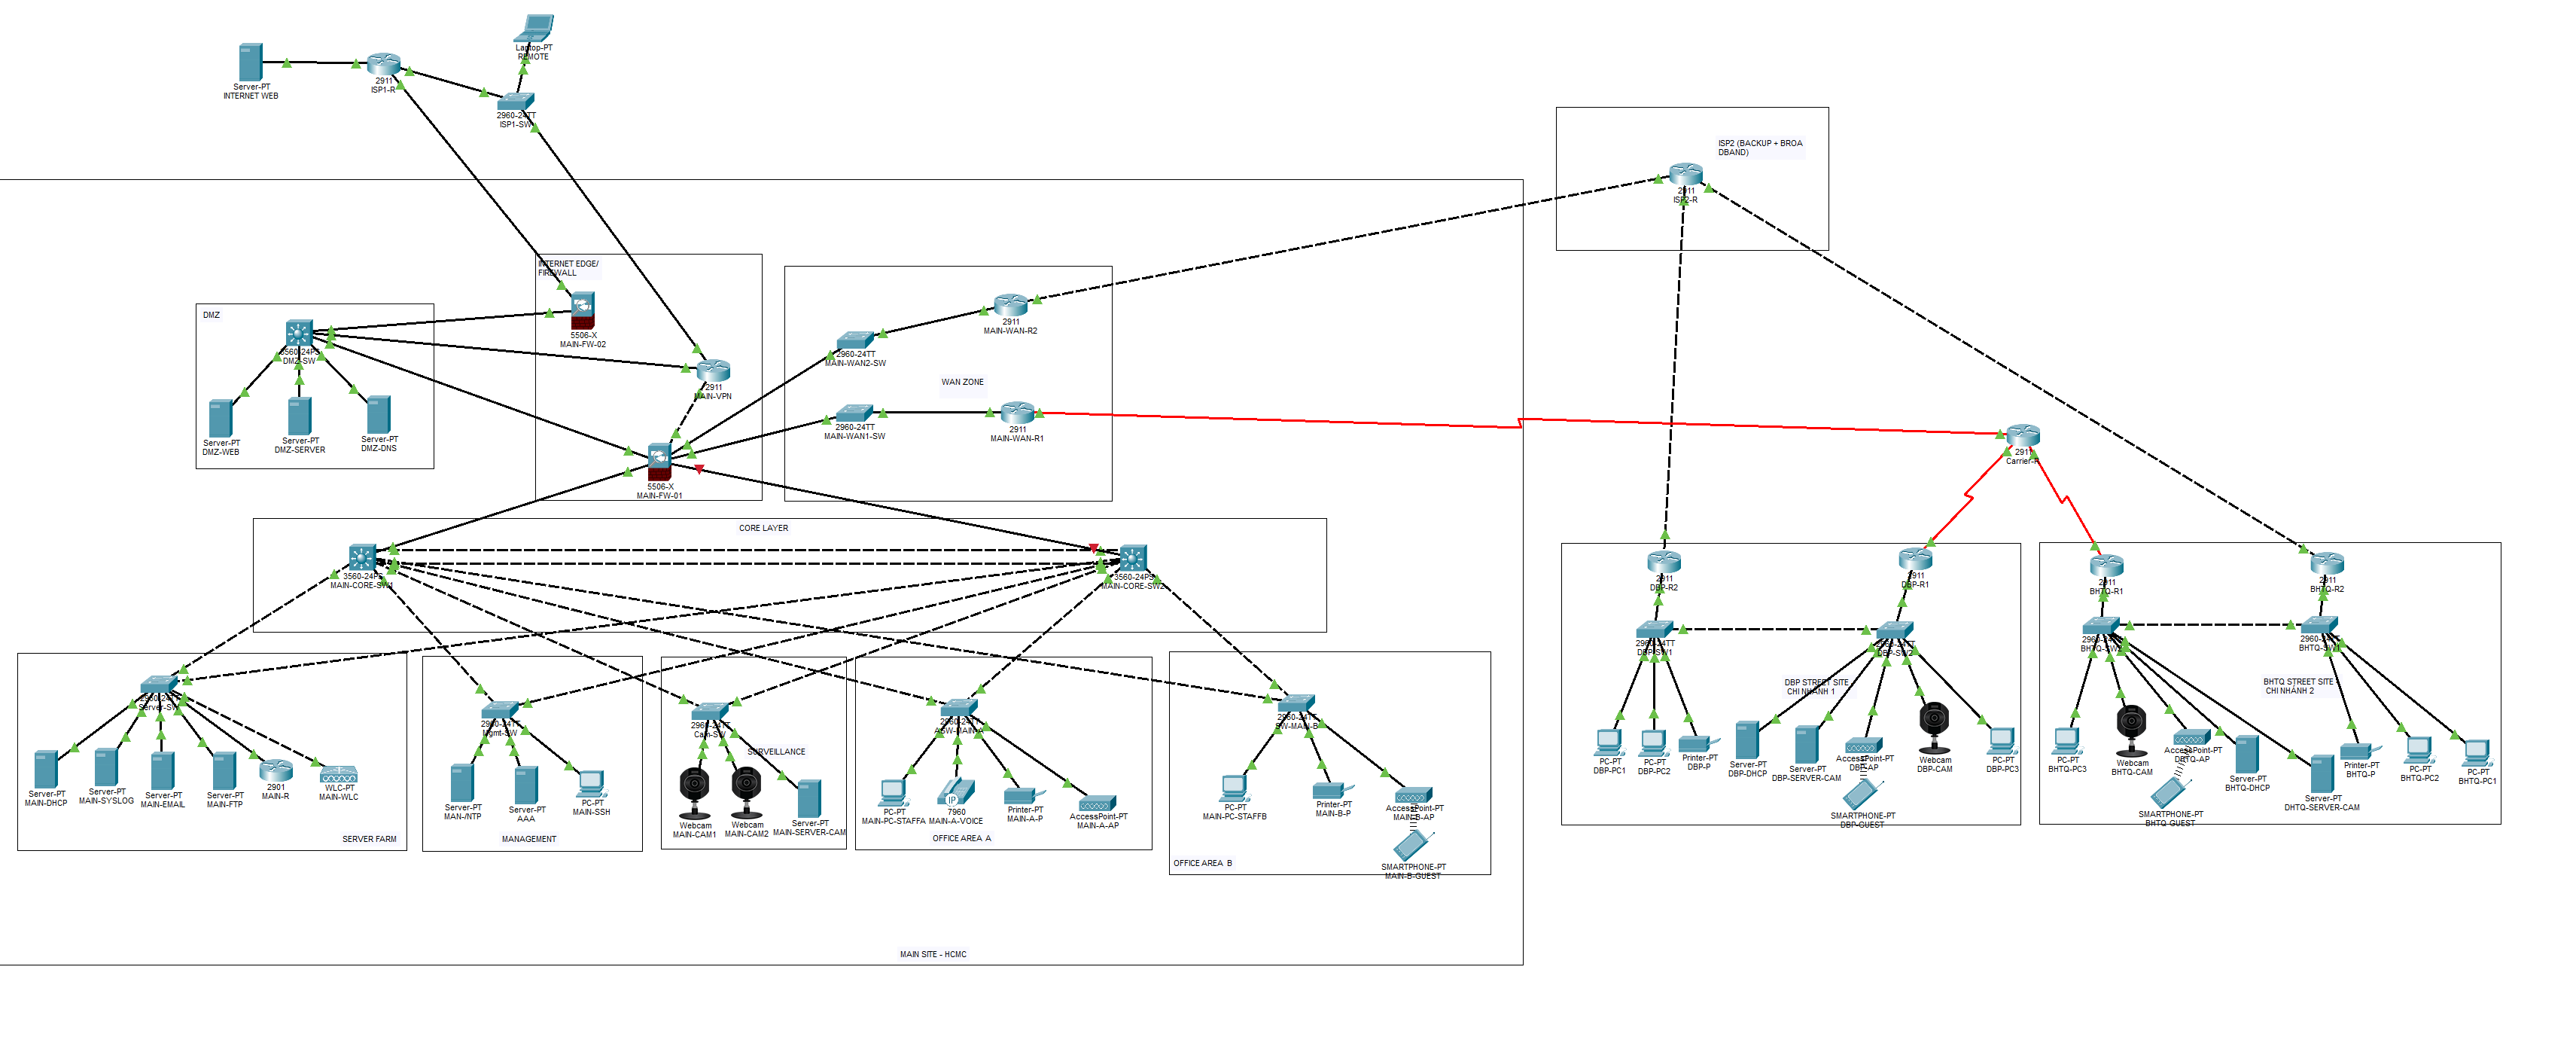
\includegraphics[width=\linewidth]{graphics/topology.png}
    \caption{Sơ đồ topology mô phỏng trên Cisco Packet Tracer (sơ đồ chuẩn)}
    \label{fig:topology}
\end{sidewaysfigure}

\subsection{Các tính năng đã mô phỏng}
\begin{small}
\setlength{\tabcolsep}{4pt}
\begin{longtable}{|p{2.2cm}|p{7.8cm}|p{3.8cm}|}
\caption{Các tính năng đã mô phỏng} \label{tab:sim_features} \\
\hline
\textbf{Nhóm} & \textbf{Tính năng} & \textbf{Thiết bị chính} \\ \hline
\endhead
Lớp 2 & VLAN, trunk 802.1Q, Rapid-PVST, LACP Port-channel 1 giữa hai Core & Core, Access \\ \hline
Dự phòng cổng & HSRP (Core: prio 200/150; chi nhánh: 110/105, \texttt{standby track Serial0/3/0}) & \texttt{MAIN-CORE-SW1/2}, \texttt{DBP/BHTQ-R1/R2} \\ \hline
Định tuyến & OSPF Area 0 (leased line, cost 10); static và default; floating static AD 150 (chi nhánh) và AD 10 (\texttt{MAIN-FW-01}) & \texttt{MAIN-WAN-R1}, \texttt{Carrier-R}, router chi nhánh \\ \hline
Firewall & Zone và security level: inside 100, inside-backup 100, wan 70, backup-wan 60, dmz 50, outside 0 & \texttt{MAIN-FW-01}, \texttt{MAIN-FW-02} \\ \hline
NAT & Static NAT \texttt{10.10.50.10} $\leftrightarrow$ \texttt{203.162.10.3} (TCP/80); PAT cho \texttt{10.0.0.0/8} ra Internet & \texttt{MAIN-FW-02} \\ \hline
ACL & \texttt{ACL-GUEST-ISOLATE} cho VLAN 60 (cần áp dụng lại, xem Bước~5 và 6) & Core \\ \hline
DHCP & Main Site: DHCP relay từ SVI tới \texttt{MAIN-DHCP}; mỗi chi nhánh có máy chủ DHCP cục bộ (\texttt{DBP-DHCP}, \texttt{BHTQ-DHCP}) & Core, \texttt{DBP-DHCP}, \texttt{BHTQ-DHCP} \\ \hline
VPN & IPsec site-to-site giữa router WAN; remote-access VPN (client nhận \texttt{10.10.200.10}) & \texttt{MAIN-WAN-R2}, \texttt{MAIN-VPN}, \texttt{REMOTE} \\ \hline
Không dây & Access Point và WLC, SSID staff và guest & Access, Server Farm (\texttt{MAIN-WLC}) \\ \hline
Giám sát & Syslog (\texttt{MAIN-SYSLOG}, \texttt{10.10.40.11}) và NTP (\texttt{MAIN-NTP}, \texttt{10.10.90.20}) & Server Farm, Management \\ \hline
\end{longtable}
\end{small}

\subsection{Cấu hình quan trọng (trích)}

\subsubsection{HSRP và tracking ở chi nhánh}
\begin{lstlisting}[language=csh,caption={Subinterface VLAN 10 trên router chính chi nhánh}]
interface GigabitEthernet0/0.10
 encapsulation dot1Q 10
 ip address 10.20.10.2 255.255.255.0
 standby version 2
 standby 10 ip 10.20.10.1
 standby 10 priority 110
 standby 10 preempt
 standby 10 track Serial0/3/0 60
\end{lstlisting}
Router R2 dùng \texttt{standby 10 priority 105} và không cần \texttt{track}.

\subsubsection{OSPF trên liên kết leased line}
\begin{lstlisting}[language=csh,caption={OSPF trên DBP-R1}]
router ospf 1
 router-id 3.3.3.1
 network 10.255.0.8 0.0.0.3 area 0
 network 10.20.0.0 0.0.255.255 area 0
!
interface Serial0/3/0
 ip ospf cost 10
\end{lstlisting}

\subsubsection{Đường dự phòng (floating static)}
\begin{lstlisting}[language=csh,caption={Floating static tại chi nhánh và route trên MAIN-FW-01}]
! Tren DBP-R2
ip route 0.0.0.0 0.0.0.0 10.255.0.17 150
! Tren MAIN-FW-01
route backup-wan 10.20.0.0 255.255.0.0 10.10.252.4 10
route wan        10.20.0.0 255.255.0.0 10.10.251.3 1
\end{lstlisting}

\subsubsection{NAT trên MAIN-FW-02}
\begin{lstlisting}[language=csh,caption={Static NAT và PAT trên MAIN-FW-02}]
object network WEB-SERVER
 host 10.10.50.10
 nat (dmz,outside) static 203.162.10.3
object network INTERNAL-NET
 subnet 10.0.0.0 255.0.0.0
 nat (dmz,outside) dynamic interface
route outside 0.0.0.0 0.0.0.0 203.162.10.1
route dmz 10.0.0.0 255.0.0.0 10.10.50.1
\end{lstlisting}
\noindent Cấu hình đầy đủ nằm trong \texttt{running-config} của các thiết bị; hostname trong cấu hình cần được đồng bộ với tên thiết bị trên sơ đồ (xem Bước~6).

\subsection{Hạn chế của Packet Tracer ảnh hưởng thiết kế}
\begin{small}
\setlength{\tabcolsep}{4pt}
\begin{longtable}{|p{3.4cm}|p{2.8cm}|p{7.4cm}|}
\caption{Hạn chế của Packet Tracer và cách xử lý} \label{tab:pt_limits} \\
\hline
\textbf{Yêu cầu thiết kế đích} & \textbf{Tình trạng trong PT} & \textbf{Cách xử lý} \\ \hline
\endhead
Failover firewall (HA) & Không có & Hai ASA độc lập, ghi vào mục vấn đề còn lại \\ \hline
IPS/IDS & Không có & Ghi trong thiết kế đích, không mô phỏng \\ \hline
Load balancer & Không có & Nhiều Server-PT hoặc DNS round-robin; ghi thuyết minh \\ \hline
SD-WAN / MPLS thật & Không có & Mô phỏng bằng leased line + floating static \\ \hline
Thiết bị y tế & Không có mô hình & VLAN 30 chỉ quy hoạch và cấu hình gateway, không có thiết bị đầu cuối \\ \hline
Subinterface trên ASA & Không dùng & Mỗi vùng một cổng vật lý (ASA 5506-X có 8 cổng) \\ \hline
\end{longtable}
\end{small}

\subsection{Tên thiết bị đầu cuối}
Báo cáo bản trước dùng nhiều tên không thống nhất cho máy đầu cuối (\texttt{PC\_DATA}, \texttt{PC-BHTQ1}, \texttt{PC-BHTQ3}, \dots). Từ bản này, tên máy đầu cuối theo sơ đồ chuẩn: \texttt{MAIN-PC-STAFFA}, \texttt{MAIN-PC-STAFFB}, \texttt{MAIN-B-GUEST}, \texttt{REMOTE}, \texttt{DBP-PC1/2/3}, \texttt{BHTQ-PC1/2/3}. Một số ảnh kiểm thử cũ vẫn hiển thị tên hoặc hostname phiên bản trước (\texttt{Core-SW1}, \texttt{WAN-R2}, \texttt{VPN-GW}); danh sách ảnh cần chụp lại nằm trong tài liệu kèm theo.

\subsection{Các lỗi mô phỏng đã xử lý}
\begin{small}
\setlength{\tabcolsep}{4pt}
\begin{longtable}{|p{3.4cm}|p{4.4cm}|p{6.0cm}|}
\caption{Các lỗi mô phỏng đã gặp và cách sửa} \label{tab:sim_errors} \\
\hline
\textbf{Lỗi} & \textbf{Nguyên nhân} & \textbf{Cách sửa} \\ \hline
\endhead
\texttt{BHTQ-R2} không thấy \texttt{10.20.40.0/24} & Default static AD 1 đè OSPF gây bất đối xứng & Đổi thành floating AD 150, bỏ \texttt{default-information originate}, \texttt{passive-interface} trên cổng broadband \\ \hline
OSPF kẹt INIT/DROTHER qua VLAN 99 & \texttt{dot1Q native} kết hợp HSRP/OSPF trên subinterface & Bỏ \texttt{native}, dùng \texttt{dot1Q 99}, native VLAN của switch về 1 \\ \hline
HSRP nhóm 90 báo Speak & Thiếu subinterface Gi0/0.90 và allowed VLAN trên trunk & Khai báo đồng bộ trên cả R1/R2, mở trunk VLAN 1, 10, 30, 40, 70, 90, 99 \\ \hline
Không tới Server BHTQ \texttt{10.30.40.10} & Server thiếu default gateway & Đặt gateway \texttt{10.30.40.1}, gán access VLAN 40 \\ \hline
\end{longtable}
\end{small}

\newpage
\section{Bước 5: Kiểm thử hệ thống bằng ping, traceroute và các công cụ khác}
\label{sec:step5}

Kết quả trong phần này lấy từ nhật ký kiểm thử của nhóm và các ảnh trong thư mục \texttt{graphics/tc\_pic}. Mục nào không có ảnh bằng chứng được đánh dấu \textbf{chưa kiểm thử}; báo cáo không ghi PASS cho ca chưa có bằng chứng. Phần bằng chứng bảo mật và VPN (SEC, DMZ, INT, VPN) được trình bày chi tiết ở mục~\ref{sec:security_test_evidence}.

\subsection{Sáu kiểm tra bắt buộc của đề bài}
\begin{small}
\setlength{\tabcolsep}{3pt}
\begin{longtable}{|c|p{2.3cm}|p{3.0cm}|p{4.6cm}|p{2.6cm}|}
\caption{Sáu kiểm tra kết nối bắt buộc} \label{tab:six_checks} \\
\hline
\textbf{\#} & \textbf{Yêu cầu} & \textbf{Lệnh} & \textbf{Kết quả ghi nhận} & \textbf{Trạng thái} \\ \hline
\endhead
1 & PC cùng VLAN & \texttt{ping} giữa hai PC cùng VLAN & Chưa có ảnh riêng & \textbf{Chưa kiểm thử} \\ \hline
2 & PC khác VLAN & \texttt{ping} từ \texttt{MAIN-PC-STAFFA} (VLAN 10) tới máy VLAN 20 và đích khác VLAN & Ảnh LAN-01: \texttt{MAIN-PC-STAFFA} ping \texttt{10.10.20.50} nhận 4/4; ảnh LAN-02: \texttt{DBP-PC1} ping \texttt{10.20.30.14} (lần đầu mất 1/4 gói, lần sau 4/4) & PASS (theo ảnh LAN-01, LAN-02) \\ \hline
3 & Main $\leftrightarrow$ chi nhánh & \texttt{ping}, \texttt{tracert 10.20.40.10} & Ảnh WAN-01 đến WAN-03: ping giữa \texttt{MAIN-PC-STAFFA}, \texttt{DBP-PC1}, \texttt{BHTQ-PC3} và máy ở site khác đều nhận 4/4; \texttt{tracert} 4 hop qua \texttt{BHTQ-R1} $\to$ \texttt{Carrier-R} $\to$ \texttt{DBP-R1} $\to$ server DBP; TC-06: 5/5, RTT 2\,ms & PASS \\ \hline
4 & Tới server DMZ & Mở \texttt{http://10.10.50.11} từ nhân viên & DMZ-01: trang hiển thị; ảnh cho thấy \texttt{10.10.50.11} là \texttt{DMZ-SERVER}, khác \texttt{DMZ-WEB} (\texttt{10.10.50.10}) & PASS \\ \hline
5 & \textbf{Khách không vào được LAN} & Ping từ \texttt{MAIN-B-GUEST} tới \texttt{10.10.20.10}, \texttt{10.10.40.10}, \texttt{10.10.50.10} & Chặn được staff và Server Farm, \textbf{nhưng ping được DMZ \texttt{10.10.50.10}} & \textbf{FAIL} (SEC-01) \\ \hline
6 & Internet tới Web server & Mở \texttt{http://192.0.2.10} từ nhân viên & INT-01: trang hiển thị & PASS \\ \hline
\end{longtable}
\end{small}

\subsection{Kiểm thử bảo mật và VPN}
Bảng~\ref{tab:security_test_summary} (mục~\ref{sec:security_test_evidence}) liệt kê các ca SEC-01, SEC-02, DMZ-01, INT-01, VPN-S2S-01, VPN-RA-01 và VPN-RA-02 cùng ảnh minh chứng. Tóm tắt:
\begin{itemize}[noitemsep,topsep=2pt]
    \item \textbf{SEC-01 (cô lập Guest): FAIL.} \texttt{MAIN-B-GUEST} bị chặn khi ping \texttt{10.10.20.10} và \texttt{10.10.40.10} nhưng vẫn ping được DMZ \texttt{10.10.50.10} (4/4) và máy ngoài \texttt{192.0.2.10} (3/4).
    \item \textbf{SEC-02:} từ \texttt{REMOTE} ping \texttt{10.10.40.10} (không qua VPN) bị timeout 4/4; PASS có giới hạn.
    \item \textbf{VPN:} IPsec site-to-site kết thúc tại \texttt{MAIN-WAN-R2} (peer \texttt{10.255.0.18}, \texttt{10.255.0.22}); VPN truy cập từ xa kết thúc tại \texttt{MAIN-VPN}, client \texttt{REMOTE} nhận \texttt{10.10.200.10}.
    \item \textbf{Chưa kiểm thử:} SSH từ Jump Host \texttt{MAIN-SSH}; Internet $\to$ DMZ qua NAT \texttt{203.162.10.3}; camera/NVR; IDS/IPS.
\end{itemize}
\noindent \textbf{Ghi chú SEC-01:} \texttt{ACL-GUEST-ISOLATE} đã được sửa trong báo cáo nhưng \textbf{chưa áp dụng vào mô phỏng và chạy lại}. Lỗi nằm ở chỗ \texttt{DMZ-WEB} \texttt{10.10.50.10} thuộc \texttt{10.0.0.0/8}; ACL phải \texttt{deny} trước khi \texttt{permit} web ra ngoài. Phải áp dụng và chạy lại trước khi ghi PASS.
\begin{lstlisting}[language=csh,caption={ACL-GUEST-ISOLATE đã sửa (chưa áp dụng vào mô phỏng)}]
ip access-list extended ACL-GUEST-ISOLATE
 permit udp any eq bootpc any eq bootps
 permit udp any host 10.10.40.10 eq domain
 permit tcp 10.10.60.0 0.0.3.255 host 10.10.40.10 eq domain
 deny   ip  10.10.60.0 0.0.3.255 10.0.0.0 0.255.255.255
 permit tcp 10.10.60.0 0.0.3.255 any eq www
 permit tcp 10.10.60.0 0.0.3.255 any eq 443
!
interface Vlan60
 ip access-group ACL-GUEST-ISOLATE in
\end{lstlisting}

\subsection{Kịch bản demo}

\subsubsection{Giai đoạn 1: Trạng thái chuẩn và hội tụ}

\paragraph{Bước 1.1: Kiểm tra HSRP.} Truy cập CLI của các thiết bị gateway chính và phụ để kiểm tra trạng thái nhóm HSRP. Hai ảnh HA-01 và HA-01.1 minh chứng cho hai switch lõi; listing cho \texttt{DBP-R1} chưa có ảnh riêng.
\begin{lstlisting}[language=csh,caption={Kiểm tra HSRP trên MAIN-CORE-SW1 và router chi nhánh}]
MAIN-CORE-SW1# show standby brief
                   P indicates configured to preempt.
Interface   Grp  Pri P State   Active          Standby         Virtual IP
Vl10        10   200 P Active  local           10.10.10.3      10.10.10.1
Vl20        20   200 P Active  local           10.10.20.3      10.10.20.1
Vl30        30   200 P Active  local           10.10.30.3      10.10.30.1
Vl40        40   200 P Active  local           10.10.40.3      10.10.40.1
Vl60        60   200 P Active  local           10.10.60.3      10.10.60.1
Vl70        70   200 P Active  local           10.10.70.3      10.10.70.1
Vl80        80   200 P Active  local           10.10.80.3      10.10.80.1
Vl90        90   200 P Active  local           10.10.90.3      10.10.90.1
Vl250       250  200 P Active  local           10.10.250.3     10.10.250.1

DBP-R1# show standby brief
Interface   Grp  Pri P State   Active          Standby         Virtual IP
Gi0/0.10    10   110 P Active  local           10.20.10.3      10.20.10.1
Gi0/0.30    30   110 P Active  local           10.20.30.3      10.20.30.1
Gi0/0.40    40   110 P Active  local           10.20.40.3      10.20.40.1
Gi0/0.70    70   110 P Active  local           10.20.70.3      10.20.70.1
Gi0/0.90    90   110 P Active  local           10.20.90.3      10.20.90.1
Gi0/0.99    99   110 P Active  local           10.20.99.3      10.20.99.1
\end{lstlisting}
\noindent \textbf{Tiêu chí nghiệm thu:} toàn bộ nhóm trên \texttt{MAIN-CORE-SW1}, \texttt{DBP-R1}, \texttt{BHTQ-R1} ở trạng thái \texttt{Active} và hiển thị đúng địa chỉ Standby của thiết bị phụ (\texttt{MAIN-CORE-SW2}, \texttt{DBP-R2}, \texttt{BHTQ-R2}); không còn nhóm Speak/Unknown.

\tcfig{HA_01.png}{HA-01: trạng thái HSRP trên MAIN-CORE-SW1 và MAIN-CORE-SW2}{fig:demo-ha-01}
\tcfig{HA_01.1.png}{HA-01.1: sơ đồ và ping liên tục từ MAIN-PC-STAFFA tới 10.10.50.12, có gián đoạn rồi phục hồi}{fig:demo-ha-01-1}

\paragraph{Bước 1.2: Kiểm tra láng giềng OSPF.}
\begin{lstlisting}[language=csh,caption={Láng giềng OSPF Area 0}]
Carrier-R# show ip ospf neighbor
Neighbor ID     Pri   State           Dead Time   Address         Interface
1.1.1.1           1   FULL/  -        00:00:32    10.255.0.2      Serial0/3/0
1.1.1.2           1   FULL/  -        00:00:35    10.255.0.6      Serial0/3/1
3.3.3.1           1   FULL/  -        00:00:31    10.255.0.10     Serial0/3/2
4.4.4.1           1   FULL/  -        00:00:33    10.255.0.14     Serial0/3/3

BHTQ-R2# show ip ospf neighbor
Neighbor ID     Pri   State           Dead Time   Address         Interface
4.4.4.1           1   FULL/DR         00:00:38    10.30.99.2      GigabitEthernet0/0.99
\end{lstlisting}
\noindent \textbf{Tiêu chí nghiệm thu:} liên kết Serial đạt \texttt{FULL/-}; liên kết subinterface đạt \texttt{FULL/DR} hoặc \texttt{FULL/BDR}.

\paragraph{Bước 1.3: Ping và truy vết đường chính.} Từ \texttt{BHTQ-PC1} (\texttt{10.30.10.10}):
\begin{lstlisting}[language=csh,caption={Ping và traceroute từ chi nhánh BHTQ}]
C:\> ping 10.10.40.10
Reply from 10.10.40.10: bytes=32 time=4ms TTL=124
Reply from 10.10.40.10: bytes=32 time=3ms TTL=124
Reply from 10.10.40.10: bytes=32 time=3ms TTL=124
Reply from 10.10.40.10: bytes=32 time=3ms TTL=124
Ping statistics for 10.10.40.10: Packets: Sent = 4, Received = 4, Lost = 0 (0% loss)

C:\> tracert 10.20.40.10
  1     1 ms     1 ms     1 ms   10.30.10.2      (BHTQ-R1)
  2     2 ms     2 ms     2 ms   10.255.0.13     (Carrier-R)
  3     3 ms     2 ms     3 ms   10.255.0.10     (DBP-R1)
  4     4 ms     3 ms     4 ms   10.20.40.10     (Server DBP)
Trace complete.
\end{lstlisting}
\noindent Các ảnh LAN-01, LAN-02 và WAN-01 đến WAN-03 dưới đây ghi nhận ping từ các máy trạm; kết quả chỉ áp dụng cho đích và lần thử hiển thị.

\tcfig{LAN_01.png}{LAN-01: MAIN-PC-STAFFA truy cập một số đích LAN và DMZ}{fig:demo-lan-01}
\tcfig{LAN_02.png}{LAN-02: DBP-PC1 ping 10.20.30.14, lần đầu mất gói rồi nhận đủ phản hồi}{fig:demo-lan-02}
\tcfig{WAN_01.png}{WAN-01: MAIN-PC-STAFFA ping 10.30.30.10 và 10.20.10.18, đều nhận đủ 4/4 phản hồi}{fig:demo-wan-01}
\tcfig{WAN_02.png}{WAN-02: BHTQ-PC3 ping 10.10.10.50 nhận đủ 4/4 phản hồi và cấu hình IP của máy}{fig:demo-wan-02}
\tcfig{WAN_03.png}{WAN-03: DBP-PC1 ping 10.20.30.14 (lần đầu mất 1/4 gói) và 10.10.10.50 nhận đủ phản hồi}{fig:demo-wan-03}

\subsubsection{Giai đoạn 2: An ninh phân vùng, DMZ và Internet}
\begin{itemize}[noitemsep,topsep=2pt]
    \item \textbf{Cô lập Guest:} từ \texttt{MAIN-B-GUEST} (VLAN 60, \texttt{10.10.60.50}), ping tới \texttt{10.10.20.10} và \texttt{10.10.40.10} không có phản hồi; ping \texttt{10.10.50.10} nhận đủ phản hồi ở lần thử sau; ping \texttt{192.0.2.10} nhận 3/4 phản hồi. Kết luận: ca cô lập Guest \textbf{FAIL} (ảnh \texttt{SEC\_01.png}).
    \item \textbf{Web DMZ:} từ \texttt{MAIN-PC-STAFFA}, mở \texttt{http://10.10.50.11} (\texttt{DMZ-SERVER}) hiển thị trang Cisco Packet Tracer (ảnh \texttt{DMZ\_01.png}).
    \item \textbf{Web Internet:} mở \texttt{http://192.0.2.10} (\texttt{INTERNET WEB}) hiển thị thành công (ảnh \texttt{INT\_01.png}).
\end{itemize}
Các ảnh này không kiểm chứng truy cập Web từ Internet vào địa chỉ NAT công khai hoặc SSH quản trị; các phép thử đó \textbf{chưa được thực hiện}.

\subsubsection{Giai đoạn 3: Chuyển đổi dự phòng WAN tại chi nhánh BHTQ}
\begin{enumerate}[noitemsep,topsep=2pt]
    \item \textbf{Luồng giám sát:} trên \texttt{BHTQ-PC3} chạy \texttt{ping 10.20.40.10 -t} tới server DBP.
    \item \textbf{Bơm sự cố đứt leased line:} trên \texttt{BHTQ-R1} ngắt cổng nối \texttt{Carrier-R}:
\begin{lstlisting}[language=csh]
BHTQ-R1(config)# interface Serial0/3/0
BHTQ-R1(config-if)# shutdown
%LINK-5-CHANGED: Interface Serial0/3/0, changed state to administratively down
%LINEPROTO-5-UPDOWN: Line protocol on Interface Serial0/3/0, changed state to down
\end{lstlisting}
    \item Bấm \texttt{Alt + D} để đẩy nhanh chu kỳ phát hiện lỗi trong mô phỏng.
    \item \textbf{Phản ứng của hệ thống:}
    \begin{itemize}[noitemsep,topsep=2pt]
        \item \textit{HSRP tracking:} \texttt{standby track Serial0/3/0 decrement 60} làm priority của \texttt{BHTQ-R1} giảm từ $110$ xuống $50$ trên toàn bộ nhóm VLAN.
        \item \textit{Preemption:} \texttt{BHTQ-R2} (priority $105 > 50$) chuyển sang \texttt{Active}.
        \item \textit{Floating static:} OSPF giữa \texttt{BHTQ-R1} và \texttt{Carrier-R} mất, tuyến \texttt{ip route 0.0.0.0 0.0.0.0 10.255.0.21 150} vào bảng định tuyến.
    \end{itemize}
    \item \textbf{Kết quả ghi nhận:} chỉ rơi \textbf{1 gói}, RTT tăng từ $3\,\text{ms}$ lên $11\,\text{ms}$ do đi qua đường broadband; \texttt{tracert} đi qua \texttt{BHTQ-R2} $\to$ \texttt{ISP2-R} $\to$ \texttt{DBP-R2} $\to$ server DBP.
\begin{lstlisting}[language=csh]
Reply from 10.20.40.10: bytes=32 time=3ms TTL=124
Request timed out.
Reply from 10.20.40.10: bytes=32 time=12ms TTL=123
Reply from 10.20.40.10: bytes=32 time=11ms TTL=123

C:\> tracert 10.20.40.10
  1     1 ms     1 ms     1 ms   10.30.10.3      (BHTQ-R2 - Active gateway moi)
  2     5 ms     4 ms     5 ms   10.255.0.21     (ISP2-R)
  3     8 ms     7 ms     7 ms   10.255.0.18     (DBP-R2)
  4     9 ms     8 ms     9 ms   10.20.40.10     (Server DBP)
\end{lstlisting}
    \item \textbf{Failback:} \texttt{no shutdown} trên \texttt{Serial0/3/0}; \texttt{BHTQ-R1} lấy lại \texttt{Active} nhờ \texttt{standby preempt}, OSPF \texttt{FULL} trở lại với \texttt{Carrier-R}.
\end{enumerate}
Các ảnh WAN-01 đến WAN-03, HA-02.1 và HA-02.2 chỉ hiển thị ping và CLI; riêng HA-02.1/HA-02.2 là CLI của \texttt{DBP-R2}. Các ảnh này \textbf{không tự chứng minh} đường dự phòng cụ thể hoặc thời gian gián đoạn.

\tcfig{HA_02.1.png}{HA-02.1: log HSRP/OSPF khi khởi động và ping 10.10.40.10 từ DBP-R2 (lần đầu 3/5, lần sau 5/5)}{fig:demo-ha-02-1}
\tcfig{HA_02.2.png}{HA-02.2: log chuyển trạng thái HSRP và ping từ DBP-R2 tới 10.10.40.10}{fig:demo-ha-02-2}

\subsubsection{Giai đoạn 4: Dự phòng lõi tại Main Site}
\begin{small}
\setlength{\tabcolsep}{4pt}
\begin{longtable}{|c|p{5.0cm}|p{4.6cm}|p{2.4cm}|}
\caption{Kiểm thử dự phòng lõi} \label{tab:core_ha} \\
\hline
\textbf{Thử nghiệm} & \textbf{Thao tác} & \textbf{Kết quả theo báo cáo} & \textbf{Bằng chứng} \\ \hline
\endhead
4.1 & \texttt{shutdown} \texttt{Fa0/2} trên \texttt{MAIN-CORE-SW1} (một cáp trong Port-channel 1), ping \texttt{10.10.40.10 -t} từ \texttt{MAIN-PC-STAFFA} & 0\% mất gói, LACP dồn lưu lượng sang cáp còn lại & Mô tả trong báo cáo, chưa có ảnh \\ \hline
4.2 & Tắt \texttt{MAIN-CORE-SW1} & \texttt{MAIN-CORE-SW2} thành \texttt{Active} (holdtime 10\,s); đường VLAN 253 lên \texttt{MAIN-FW-01} Gi1/5 được thiết kế làm tuyến dự phòng & \textbf{Chưa kiểm chứng}: liên kết down trên sơ đồ, chưa có ảnh \\ \hline
\end{longtable}
\end{small}
\noindent Khi chạy thử 4.2 cần bỏ \texttt{shutdown} trên \texttt{Gi1/5} của \texttt{MAIN-FW-01} (cấu hình hiện đang shutdown). Kết quả mong đợi của 4.2 là hoạt động truy cập dịch vụ Server Farm vẫn liên tục, nhưng điều này chưa được xác nhận.

\subsection{Bảng nghiệm thu TC-01 đến TC-06}
\begin{small}
\setlength{\tabcolsep}{3pt}
\begin{longtable}{|c|p{2.5cm}|p{2.2cm}|c|p{5.4cm}|}
\caption{Bảng kết quả kiểm thử TC-01 đến TC-06} \label{tab:test_matrix} \\
\hline
\textbf{Mã} & \textbf{Hạng mục} & \textbf{Ban đầu} & \textbf{Kết quả} & \textbf{Nguyên nhân và xử lý} \\ \hline
\endfirsthead
\hline \textbf{Mã} & \textbf{Hạng mục} & \textbf{Ban đầu} & \textbf{Kết quả} & \textbf{Nguyên nhân và xử lý} \\ \hline
\endhead
TC-01 & Định tuyến \texttt{BHTQ-R2} tới server DBP \texttt{10.20.40.10} & Mất 100\% (0/5) & PASS & Default static AD 1 đè OSPF gây bất đối xứng. Đổi thành floating AD 150, bỏ \texttt{default-information originate}, đặt \texttt{passive-interface} trên cổng broadband. \\ \hline
TC-02 & Láng giềng OSPF qua VLAN 99 (BHTQ) & Kẹt INIT/DROTHER & PASS & Lệch thẻ do \texttt{dot1Q native} kết hợp HSRP/OSPF. Bỏ \texttt{native}, dùng \texttt{dot1Q 99}, native VLAN switch về 1, xóa tiến trình OSPF. \\ \hline
TC-03 & Bảng MAC trên trunk VLAN 99 & Học đủ MAC của R1 và R2 & PASS & L2 ổn định, không vòng STP, không khóa Port-Security. \\ \hline
TC-04 & Đồng bộ HSRP nhóm 90 và 99 & Nhóm 90 báo Speak & PASS & Thiếu \texttt{Gi0/0.90}, \texttt{Gi0/0.99} và allowed VLAN trên trunk. Khai báo đồng bộ trên R1/R2, mở trunk VLAN 1, 10, 30, 40, 70, 90, 99. \\ \hline
TC-05 & Traceroute DBP sang server BHTQ \texttt{10.30.40.10} & Rớt hop 4 & PASS & Server thiếu gateway. Đặt \texttt{10.30.40.1}, gán access VLAN 40. \\ \hline
TC-06 & Ping trực tiếp qua leased line & 5/5, RTT 2\,ms & PASS & Tuyến chính qua \texttt{Carrier-R} ổn định, được ưu tiên khi không có sự cố. \\ \hline
\end{longtable}
\end{small}
\noindent Chỉ các cấu hình đã xuất (15 thiết bị) mới được xác nhận là đã lưu; chưa chứng minh đã sao lưu đủ toàn bộ thiết bị hoặc đã kiểm thử đầy đủ ACL/NAT. Bằng chứng khắc phục native VLAN hiện ghi nhận tại BHTQ; cấu hình tương ứng tại DBP cần kiểm tra riêng.

\subsection{Việc cần làm để hoàn thiện kiểm thử}
\begin{enumerate}[noitemsep,topsep=2pt]
    \item Sửa và chạy lại SEC-01 (áp dụng ACL vào \texttt{Vlan60}).
    \item Chạy thêm: ping cùng VLAN, Internet $\to$ DMZ qua \texttt{203.162.10.3}, SSH từ \texttt{MAIN-SSH}, camera $\to$ NVR, thử nghiệm 4.2.
    \item Chụp ảnh từng ca với mã trùng bảng trong báo cáo (ví dụ \texttt{LAN-01}).
    \item Không ghi PASS cho ca chưa có ảnh bằng chứng.
\end{enumerate}

\newpage
\section{Bước 6: Đánh giá lại thiết kế, vấn đề còn lại và định hướng phát triển}
\label{sec:step6}

\subsection{Đánh giá theo tiêu chí}
\begin{small}
\setlength{\tabcolsep}{3pt}
\begin{longtable}{|p{2.2cm}|p{4.6cm}|p{4.8cm}|p{1.9cm}|}
\caption{Đánh giá thiết kế theo các tiêu chí của đề bài} \label{tab:evaluation} \\
\hline
\textbf{Tiêu chí} & \textbf{Đã đạt} & \textbf{Còn hạn chế} & \textbf{Đánh giá} \\ \hline
\endfirsthead
\hline \textbf{Tiêu chí} & \textbf{Đã đạt} & \textbf{Còn hạn chế} & \textbf{Đánh giá} \\ \hline
\endhead
\textbf{Độ tin cậy (HA)} & Core đôi + HSRP + LACP (thử nghiệm 4.1: 0\% mất gói); chi nhánh 2 router HSRP + \texttt{standby track}; WAN chính/phụ; failover BHTQ rơi 1 gói & Firewall không HA (hai ASA độc lập); \texttt{DMZ-SW} là điểm hỏng đơn; một ISP phía Internet; \texttt{Server-SW}, \texttt{Mgmt-SW}, \texttt{Cam-SW} chỉ có một switch; tuyến VLAN 253 chưa kiểm chứng & Khá \\ \hline
\textbf{Dễ nâng cấp, mở rộng} & Subnet dư (\texttt{/23}, \texttt{/22}); tóm tắt \texttt{/16} theo site; cấu trúc module & VLAN 10 chi nhánh \texttt{/24} không đủ 260 máy ($+20\%$); chưa dùng quản trị tập trung/automation & Khá \\ \hline
\textbf{Phần mềm hỗ trợ đa dạng} & Server Farm VLAN 40 cho các dịch vụ hạ tầng; DMZ cho web/DNS; thoại IP (VLAN 80) & Chưa kiểm thử ứng dụng thật; HIS, RIS--PACS, LIS, CRM không được mô phỏng; Packet Tracer chỉ mô phỏng dịch vụ cơ bản (HTTP, DNS, DHCP, email) & Trung bình \\ \hline
\textbf{An toàn (safety)} & Camera VLAN 70 riêng; Medical VLAN 30 được quy hoạch riêng; nguồn điện và làm mát nêu ở checklist Bước~1 & Chưa mô phỏng UPS, chống sét, kiểm soát ra vào (thuộc khảo sát vật lý); VLAN 30 không có thiết bị y tế trong Packet Tracer & Chưa kiểm chứng \\ \hline
\textbf{Bảo mật mạng} & Hai tầng firewall, DMZ, NAT/PAT, security level theo zone, IPsec site-to-site và remote-access VPN, VLAN quản trị & \textbf{Guest vẫn ping được DMZ (SEC-01 FAIL)}; DMZ cho phép rộng; chưa có IDS/IPS (PT không hỗ trợ); ACL quản trị chưa áp dụng đầy đủ; chưa có AAA/802.1X thực tế & Cần cải thiện \\ \hline
\textbf{Hiệu năng} & Tính băng thông theo Bước~3; EtherChannel & Chưa có QoS đã kiểm thử; chưa đo throughput & Chưa kiểm chứng \\ \hline
\end{longtable}
\end{small}

\subsection{Vấn đề còn lại của dự án}

\subsubsection{Lỗi và điểm yếu đã biết}
\begin{small}
\setlength{\tabcolsep}{3pt}
\begin{longtable}{|c|p{4.3cm}|p{3.4cm}|p{5.0cm}|}
\caption{Các vấn đề còn lại và hướng xử lý} \label{tab:open_issues} \\
\hline
\textbf{\#} & \textbf{Vấn đề} & \textbf{Hậu quả} & \textbf{Hướng xử lý} \\ \hline
\endfirsthead
\hline \textbf{\#} & \textbf{Vấn đề} & \textbf{Hậu quả} & \textbf{Hướng xử lý} \\ \hline
\endhead
1 & Guest ping được \texttt{10.10.50.10} (SEC-01) & Vi phạm yêu cầu khách không truy cập LAN/DMZ & Áp dụng \texttt{ACL-GUEST-ISOLATE} (có \texttt{deny 10.0.0.0/8} trước \texttt{permit web}) lên \texttt{Vlan60}, chạy lại \\ \hline
2 & \texttt{DMZ-SW} là điểm hỏng đơn giữa hai firewall & Mất DMZ và đường Internet $\leftrightarrow$ nội bộ & Thêm switch thứ hai hoặc dùng EtherChannel; hoặc ghép hai ASA thành cặp HA (thiết bị thật) \\ \hline
3 & DMZ cho phép lưu lượng rộng & DMZ bị khai thác có thể đi sâu vào mạng & Chỉ cho phép đúng luồng (HTTP/HTTPS tới Web, DNS), chặn mặc định DMZ $\to$ inside \\ \hline
4 & Một số ACL đã viết nhưng chưa gắn vào interface & Chính sách không có hiệu lực & Gắn \texttt{ip access-group}/\texttt{access-group}, kiểm tra bộ đếm \texttt{show access-lists} \\ \hline
5 & Lỗi/khác biệt route trên \texttt{MAIN-FW-01} (next-hop, \texttt{route wan}/\texttt{backup-wan}) & Đường dự phòng có thể không như thiết kế & Kiểm tra \texttt{show route}, thử tắt đường chính \\ \hline
6 & Trộn OSPF và định tuyến tĩnh/mặc định & Định tuyến bất đối xứng, firewall mất state & Dùng AD nhất quán; mọi đường dự phòng là floating static; redistribute có kiểm soát \\ \hline
7 & Chỉ có một ISP phía Internet (\texttt{ISP1-R}) & Không đạt yêu cầu 2$\times$DSL có load-balancing của đề bài & Thêm ISP thứ hai + PBR/ECMP hoặc SLA tracking trên \texttt{MAIN-FW-02} (thiết kế đích) \\ \hline
8 & VLAN 10 chi nhánh \texttt{/24} (254 host) so với 260 máy $+20\% = 312$ & Cạn địa chỉ & Đổi sang \texttt{/23} hoặc tách thêm VLAN \\ \hline
9 & Không có load balancer, IPS/IDS, phát hiện phishing trong Packet Tracer & Không đạt đầy đủ yêu cầu bảo mật cao & Nêu trong thiết kế đích: Firepower, WAF/LB, email gateway \\ \hline
10 & Liên kết \texttt{inside-backup} (\texttt{Gi1/5}, VLAN 253) đang shutdown/down & Chưa kiểm thử được failover khi \texttt{MAIN-CORE-SW1} hỏng & \texttt{no shutdown}, kiểm thử thử nghiệm 4.2 và chụp ảnh \\ \hline
11 & Khác biệt giữa báo cáo, sơ đồ và cấu hình (DHCP chi nhánh: máy chủ cục bộ so với \texttt{ip helper-address}; địa chỉ \texttt{logging}; decrement track; native VLAN 99; cổng Serial của \texttt{MAIN-WAN-R2}) & Tài liệu và mô phỏng không đồng nhất & Đối chiếu với tệp mô phỏng rồi sửa một nơi \\ \hline
12 & Hostname trong cấu hình (\texttt{ASA1}, \texttt{ASA2}, \texttt{Core-SW1/2}, \texttt{WAN-R1/R2}, \dots) chưa trùng tên trên sơ đồ; một số ảnh kiểm thử còn nhãn phiên bản cũ & Báo cáo khó đọc, ảnh không khớp sơ đồ & Đặt \texttt{hostname MAIN-FW-01}\dots; chụp lại ảnh theo danh sách kèm theo \\ \hline
\end{longtable}
\end{small}

\subsubsection{Phạm vi chưa làm (talented engineer)}
Đề yêu cầu cho chương trình talented engineer: kế hoạch bảo mật, ACL, IDS/IPS và hướng dẫn best practice. Hiện đã có kế hoạch, ACL và VPN (phần~\ref{sec:security_architecture}); \textbf{chưa có IDS/IPS} và best-practice guide hoàn chỉnh.

\subsection{Định hướng phát triển}
\begin{small}
\setlength{\tabcolsep}{4pt}
\begin{longtable}{|p{2.2cm}|p{11.6cm}|}
\caption{Định hướng phát triển} \label{tab:roadmap} \\
\hline
\textbf{Giai đoạn} & \textbf{Hạng mục} \\ \hline
\endhead
Ngắn hạn & Sửa SEC-01; gắn các ACL; thống nhất tên thiết bị và hostname; hoàn thiện kiểm thử Bước~5; bổ sung bằng chứng \\ \hline
Trung hạn & Firewall HA (Active/Standby); hai nhà mạng Internet; QoS; 802.1X + RADIUS; Syslog/SNMP tập trung \\ \hline
Dài hạn & SD-WAN thay hoặc bổ sung leased line; IPS/IDS (Firepower); WAF + load balancer; NAC; tự động hóa cấu hình (Ansible); 10/40\,GbE cho Core và hệ thống PACS \\ \hline
\end{longtable}
\end{small}

\subsection{Kết luận}
Thiết kế đạt phần lớn yêu cầu về phân cấp, dự phòng, phân vùng và WAN. Các điểm cần xử lý trước khi nộp là: \textbf{SEC-01}; các kiểm thử còn thiếu (cùng VLAN, Internet $\to$ DMZ qua NAT, SSH, camera, dự phòng lõi qua VLAN 253); và tính đồng nhất giữa báo cáo, sơ đồ và tệp mô phỏng. Các yêu cầu IPS/IDS, load balancer, HA firewall và hai ISP được trình bày như \textbf{thiết kế đích}, không phải kết quả mô phỏng.

\newpage
\section{Thiết kế bảo mật và kiểm soát truy cập}
\label{sec:security_architecture}

\subsection{Mục đích, phạm vi và nguồn thiết kế}
Phần này trình bày đánh giá và đề xuất kiểm soát bảo mật cho topology cuối cùng được mô tả trong báo cáo, gồm Main Site, DBP và BHTQ. Các VLAN, subnet, thiết bị biên và luồng WAN trong phần này được đồng bộ theo mục quy hoạch và cấu hình mô phỏng của báo cáo; các khuyến nghị bảo mật được phân biệt với những gì báo cáo ghi nhận là đã cấu hình hoặc kiểm thử. Ma trận truy cập, hướng dẫn ACL và test plan là các sản phẩm chi tiết đi kèm.

Không gian địa chỉ tổng là Main \texttt{10.10.0.0/16}, DBP \texttt{10.20.0.0/16}, BHTQ \texttt{10.30.0.0/16}; các liên kết WAN dùng các subnet point-to-point trong \texttt{10.255.0.0/24}. Dải \texttt{/16} là không gian địa chỉ tổng của mỗi cơ sở, không phải subnet đầu cuối dùng chung.

\subsection{Tài sản và đánh giá rủi ro ban đầu}
Mức đánh giá dưới đây là ưu tiên thiết kế định tính, cần được chủ sở hữu hệ thống và nhóm xác nhận; không thay thế khảo sát chuyên sâu hoặc phân tích mối đe dọa.

\begin{small}
\setlength{\tabcolsep}{3pt}
\begin{longtable}{|p{2.6cm}|p{3.3cm}|p{2.7cm}|p{5.8cm}|}
\caption{Tài sản trọng yếu, rủi ro và biện pháp bảo vệ} \label{tab:security_assets_risks} \\
\hline
\textbf{Tài sản/vùng} & \textbf{Vị trí theo topology báo cáo} & \textbf{Mức quan trọng} & \textbf{Rủi ro và hướng bảo vệ} \\ \hline
\endfirsthead
\multicolumn{4}{c}{{\bfseries Bảng \thetable\ -- tiếp theo từ trang trước}} \\
\hline
\textbf{Tài sản/vùng} & \textbf{Vị trí theo topology báo cáo} & \textbf{Mức quan trọng} & \textbf{Rủi ro và hướng bảo vệ} \\ \hline
\endhead
\hline
\multicolumn{4}{|r|}{{\textit{Xem tiếp ở trang sau...}}} \\ \hline
\endfoot
\hline
\endlastfoot

HIS, RIS-PACS, LIS, CRM và cơ sở dữ liệu & Server Farm Main, VLAN 40 & Rất cao & Truy cập trái phép, rò rỉ hoặc sửa dữ liệu bệnh nhân; giới hạn nguồn và đích theo dịch vụ, phân quyền ứng dụng, bảo vệ dữ liệu và kiểm thử khôi phục bản sao lưu. \\ \hline
Máy chủ chi nhánh & VLAN Server 40 tại DBP/BHTQ & Cao & Truy cập trái phép hoặc lan truyền sự cố giữa các cơ sở; chỉ cho phép luồng nghiệp vụ/quản trị đã duyệt và ghi nhật ký phiên truy cập. \\ \hline
Thiết bị y tế kết nối mạng & VLAN 30 tại từng cơ sở & Rất cao & Thiết bị cũ hoặc khó cập nhật có thể bị xâm nhập, ảnh hưởng dịch vụ lâm sàng; phân vùng riêng và xác nhận giao thức với nhà sản xuất trước khi mở quy tắc. \\ \hline
Máy trạm nhân viên & Main VLAN 10/20; DBP/BHTQ VLAN 10 & Cao & Mã độc hoặc tài khoản bị chiếm quyền có thể lan tới Server Farm; giới hạn quyền theo ứng dụng, bảo vệ tài khoản và ghi nhật ký. \\ \hline
Web và dịch vụ công khai & DMZ Main, VLAN 50 & Cao & Dịch vụ bị khai thác làm bàn đạp vào mạng nội bộ; chỉ công bố máy chủ/dịch vụ được duyệt và mặc định chặn kết nối khởi tạo từ DMZ tới LAN. \\ \hline
Wi-Fi khách & Guest Main, VLAN 60 & Trung bình & Thiết bị khách truy cập trái phép LAN hoặc gây quá tải; chỉ cho phép dịch vụ Internet được phê duyệt và cô lập khỏi các vùng nội bộ. \\ \hline
AP/WLC và SSID không dây & AP tại các cơ sở; Guest Main VLAN 60 & Cao & Cấu hình sai SSID/VLAN hoặc chiếm quyền AP/WLC; giữ Guest tách khỏi mạng nhân viên, ánh xạ Staff Wi-Fi chưa nêu trong báo cáo. \\ \hline
Camera/NVR & VLAN 70 tại Main, DBP và BHTQ & Cao & Thiết bị IoT bị chiếm quyền hoặc rò rỉ video; chỉ cho phép camera kết nối tới NVR/kho lưu trữ đã xác nhận và mặc định chặn lưu lượng ra Internet. \\ \hline
Thiết bị mạng và hệ thống quản trị & VLAN 90 tại Main, DBP và BHTQ & Rất cao & Lộ thông tin quản trị hoặc thay đổi trái phép ảnh hưởng toàn mạng; chỉ cho phép máy quản trị được duyệt qua SSH và lưu nhật ký. \\ \hline
Firewall, Edge Router và WAN & Thiết bị biên tại Main; WAN liên cơ sở & Rất cao & Cấu hình sai, xâm nhập biên hoặc sự cố đường truyền làm gián đoạn dịch vụ; rà soát thay đổi, giới hạn luồng và kiểm thử chuyển đổi dự phòng. \\ \hline
Nhật ký và bằng chứng kiểm thử & Hệ thống ghi nhật ký/nhóm dự án & Cao & Thiếu nhật ký làm chậm phát hiện/điều tra; đồng bộ thời gian, giới hạn quyền đọc/sửa và lưu bằng chứng theo quy định nhóm. \\ \hline
\end{longtable}
\end{small}

\begin{small}
\setlength{\tabcolsep}{3pt}
\begin{longtable}{|p{4.0cm}|p{2.1cm}|p{2.1cm}|p{6.2cm}|}
\caption{Tóm tắt các rủi ro ưu tiên} \label{tab:security_risk_priority} \\
\hline
\textbf{Tình huống} & \textbf{Khả năng} & \textbf{Tác động} & \textbf{Ưu tiên xử lý kiến trúc} \\ \hline
\endfirsthead
\multicolumn{4}{c}{{\bfseries Bảng \thetable\ -- tiếp theo từ trang trước}} \\
\hline
\textbf{Tình huống} & \textbf{Khả năng} & \textbf{Tác động} & \textbf{Ưu tiên xử lý kiến trúc} \\ \hline
\endhead
\hline
\multicolumn{4}{|r|}{{\textit{Xem tiếp ở trang sau...}}} \\ \hline
\endfoot
\hline
\endlastfoot

Guest hoặc thiết bị cá nhân truy cập trái phép mạng nội bộ & Trung bình & Cao & Cao: cô lập Guest, chỉ cho Internet và kiểm thử các luồng bị chặn. \\ \hline
Máy trạm nhân viên bị mã độc/chiếm tài khoản & Trung bình & Rất cao & Cao: giới hạn truy cập theo nghiệp vụ, bảo vệ quản trị và lưu log. \\ \hline
Dịch vụ công khai hoặc máy chủ DMZ bị khai thác & Trung bình & Rất cao & Cao: tách DMZ, chỉ mở dịch vụ công khai được duyệt, chặn DMZ khởi tạo kết nối vào LAN. \\ \hline
Lây nhiễm ngang giữa các cơ sở qua WAN & Trung bình & Cao & Cao: kiểm soát luồng liên cơ sở và chốt phương án OSPF/IPsec trước khi triển khai. \\ \hline
Thiết bị y tế khó cập nhật bị xâm nhập & Trung bình & Rất cao & Cao: tách Medical, chỉ mở đích/cổng có xác nhận của nhà sản xuất và chủ ứng dụng. \\ \hline
Camera/NVR bị chiếm quyền hoặc rò rỉ video & Trung bình & Cao & Cao: cô lập camera, giới hạn tới NVR/kho lưu trữ, mặc định chặn Internet. \\ \hline
Lộ thông tin quản trị hoặc cấu hình sai tường lửa/WAN & Thấp--trung bình & Rất cao & Cao: giới hạn nguồn quản trị, rà soát thay đổi, kiểm thử chuyển đổi dự phòng và lưu bằng chứng. \\ \hline
Thiếu nhật ký hoặc Wi-Fi khách quá tải & Trung bình & Trung bình--cao & Trung bình: xác định nguồn/thời hạn lưu nhật ký; giữ mạng khách tách biệt và chốt yêu cầu giới hạn tải nếu cần. \\ \hline
\end{longtable}
\end{small}

\subsection{Các vùng bảo mật theo topology cuối cùng trong báo cáo}
Bảng~\ref{tab:security_zones_report} đồng bộ VLAN/subnet với quy hoạch và cấu hình mô phỏng được trình bày trong báo cáo. Mức tin cậy là đánh giá thiết kế, không phải thuộc tính bảo đảm của VLAN.

\begin{small}
\setlength{\tabcolsep}{3pt}
\begin{longtable}{|p{2.2cm}|p{3.8cm}|p{1.5cm}|p{3.4cm}|p{3.3cm}|}
\caption{Các vùng bảo mật, địa chỉ chuẩn và mục đích bảo vệ} \label{tab:security_zones_report} \\
\hline
\textbf{Vùng bảo mật} & \textbf{VLAN/subnet theo báo cáo} & \textbf{Mức tin cậy} & \textbf{Thành phần/mục đích} & \textbf{Nguyên tắc phân tách} \\ \hline
\endfirsthead
\multicolumn{5}{c}{{\bfseries Bảng \thetable\ -- tiếp theo từ trang trước}} \\
\hline
\textbf{Vùng bảo mật} & \textbf{VLAN/subnet theo báo cáo} & \textbf{Mức tin cậy} & \textbf{Thành phần/mục đích} & \textbf{Nguyên tắc phân tách} \\ \hline
\endhead
\hline
\multicolumn{5}{|r|}{{\textit{Xem tiếp ở trang sau...}}} \\ \hline
\endfoot
\hline
\endlastfoot

Staff LAN -- Main & VLAN 10 \texttt{10.10.10.0/23}; VLAN 20 \texttt{10.10.20.0/23} & Trung bình & Máy trạm nhân viên tại hai tòa nhà & Chỉ tới ứng dụng và dịch vụ được duyệt; không quản trị thiết bị hoặc truy cập trực tiếp cơ sở dữ liệu. \\ \hline
Staff LAN -- DBP & VLAN 10 \texttt{10.20.10.0/24} & Trung bình & Máy trạm nhân viên DBP & Chỉ tới dịch vụ nghiệp vụ được duyệt qua WAN. \\ \hline
Staff LAN -- BHTQ & VLAN 10 \texttt{10.30.10.0/24} & Trung bình & Máy trạm nhân viên BHTQ & Chỉ tới dịch vụ nghiệp vụ được duyệt qua WAN. \\ \hline
Medical -- Main & VLAN 30 \texttt{10.10.30.0/24} & Thấp--trung bình & Thiết bị y tế & Chỉ cho phép luồng lâm sàng đã được khảo sát và duyệt. \\ \hline
Medical -- DBP & VLAN 30 \texttt{10.20.30.0/24} & Thấp--trung bình & Thiết bị y tế & Chỉ cho phép luồng lâm sàng đã được khảo sát và duyệt. \\ \hline
Medical -- BHTQ & VLAN 30 \texttt{10.30.30.0/24} & Thấp--trung bình & Thiết bị y tế & Chỉ cho phép luồng lâm sàng đã được khảo sát và duyệt. \\ \hline
Server Farm -- Main & VLAN 40 \texttt{10.10.40.0/24} & Cao & HIS, LIS, DB, CRM và dịch vụ cập nhật & Tách dịch vụ ứng dụng/cơ sở dữ liệu theo máy chủ và cổng; không công bố trực tiếp ra Internet. \\ \hline
Server -- DBP & VLAN 40 \texttt{10.20.40.0/24} & Cao & Hai máy chủ chi nhánh theo báo cáo & Chỉ mở dịch vụ ứng dụng/quản trị được duyệt. \\ \hline
Server -- BHTQ & VLAN 40 \texttt{10.30.40.0/24} & Cao & Hai máy chủ chi nhánh theo báo cáo & Chỉ mở dịch vụ ứng dụng/quản trị được duyệt. \\ \hline
DMZ -- Main & VLAN 50 \texttt{10.10.50.0/24} & Thấp & Web và dịch vụ công khai & Chặn kết nối khởi tạo vào LAN; chỉ công bố máy chủ/dịch vụ sau khi xác nhận. \\ \hline
Guest Wi-Fi -- Main & VLAN 60 \texttt{10.10.60.0/22} & Rất thấp & Wi-Fi khách, chỉ phục vụ Internet & Cô lập khỏi mạng nội bộ; chỉ cho phép lưu lượng ra Internet đã duyệt. \\ \hline
Camera -- Main & VLAN 70 \texttt{10.10.70.0/24} & Thấp & Camera/NVR; vị trí NVR cần xác nhận & Chỉ cho phép camera tới NVR/kho lưu trữ được duyệt; mặc định chặn Internet. \\ \hline
Voice -- Main & VLAN 80 \texttt{10.10.80.0/24} & Trung bình & Điện thoại IP nội bộ & Chỉ cho phép dịch vụ thoại và quản trị được xác định; áp dụng QoS theo cấu hình. \\ \hline
Management -- Main & VLAN 90 \texttt{10.10.90.0/24} & Cao & Quản trị thiết bị mạng & Chỉ máy quản trị được ủy quyền qua SSH. \\ \hline
Management -- DBP & VLAN 90 \texttt{10.20.90.0/24} & Cao & Quản trị thiết bị DBP & Chỉ máy quản trị được ủy quyền qua SSH. \\ \hline
Management -- BHTQ & VLAN 90 \texttt{10.30.90.0/24} & Cao & Quản trị thiết bị BHTQ & Chỉ máy quản trị được ủy quyền qua SSH. \\ \hline
Camera -- DBP & VLAN 70 \texttt{10.20.70.0/24} & Thấp & Camera chi nhánh & Chỉ cho phép luồng tới máy chủ ghi hình/quản lý được xác định. \\ \hline
Camera -- BHTQ & VLAN 70 \texttt{10.30.70.0/24} & Thấp & Camera chi nhánh & Chỉ cho phép luồng tới máy chủ ghi hình/quản lý được xác định. \\ \hline
VLAN điều khiển -- DBP/BHTQ & VLAN 99 \texttt{10.20.99.0/24}, \texttt{10.30.99.0/24} & Trung bình & Mạng kết nối định tuyến/HSRP theo mô phỏng & Không dùng làm VLAN quản trị; trunk native được đặt ở VLAN 1 theo phần kiểm thử. \\ \hline
Transit -- Main & VLAN 250 \texttt{10.10.250.0/29}; VLAN 253 \texttt{10.10.253.0/29} & Cao & Kết nối Core tới ASA1 và đường dự phòng & Chỉ cho phép lưu lượng cần thiết giữa Core và Firewall; không dùng làm mạng đầu cuối. \\ \hline
WAN chính -- Carrier-R & \texttt{10.255.0.0/30}, \texttt{10.255.0.4/30}, \texttt{10.255.0.8/30}, \texttt{10.255.0.12/30} & Trung bình & Các liên kết WAN chính theo sơ đồ & Chỉ cho phép OSPF giữa các router ngang hàng đã xác định. \\ \hline
WAN dự phòng -- ISP2-R & \texttt{10.255.0.16/30}, \texttt{10.255.0.20/30}, \texttt{10.255.0.24/30} & Trung bình & Các liên kết WAN dự phòng & Chỉ dùng khi tuyến leased line chính không khả dụng. \\ \hline
\end{longtable}
\end{small}

\noindent Tại DBP/BHTQ, VLAN 99 được dùng cho liên kết định tuyến/HSRP và trunk dùng VLAN 1 làm native; cấu hình Main giữ VLAN 99 làm native lớp 2, không có subnet/gateway và không phải VLAN quản trị. Việc khắc phục native VLAN đã được kiểm chứng tại BHTQ; DBP cần kiểm tra riêng. Mạng Guest và Camera tại Main giữ nguyên VLAN 60/70. Địa chỉ \texttt{10.255.0.0/30}, \texttt{10.255.0.4/30}, \texttt{10.255.0.8/30}, \texttt{10.255.0.12/30} là các liên kết Carrier-R; \texttt{10.255.0.16/30}, \texttt{10.255.0.20/30}, \texttt{10.255.0.24/30} là các liên kết dự phòng ISP2-R.

\subsection{Nguyên tắc phân vùng}
\begin{enumerate}
    \item Phân vùng theo chức năng và mức độ tin cậy; không mặc định cho phép truy cập giữa các mạng thuộc cùng một cơ sở.
    \item Cô lập mạng Wi-Fi khách khỏi mạng nội bộ; tách DMZ khỏi Server Farm; bảo vệ riêng Medical, Camera và Management.
    \item Chỉ mở luồng liên vùng/liên cơ sở theo nhu cầu nghiệp vụ được xác nhận, gồm nguồn, đích, giao thức/cổng và hướng khởi tạo.
    \item Tại Main, ASA2 thực hiện NAT/PAT ra ISP1; tại chi nhánh, ISP2-R là tuyến dự phòng khi leased line mất kết nối. Không mô tả Internet chi nhánh như một tuyến bắt buộc đi qua Main.
    \item Mặc định từ chối các luồng liên vùng và lưu lượng ra Internet chưa có quy tắc cho phép cụ thể. Ngoại lệ nghiệp vụ phải được chủ dịch vụ duyệt.
    \item Tách rõ cấu hình được mô tả trong báo cáo, khuyến nghị bảo mật và nội dung chưa có bằng chứng kiểm thử.
\end{enumerate}

\subsection{Tóm tắt ma trận kiểm soát truy cập}
Ma trận đầy đủ gồm các quy tắc AC-01--AC-24 trong \texttt{access\_control\_matrix.csv}; bảng~\ref{tab:security_matrix_summary} tóm tắt các luồng chính theo topology trong báo cáo. Chỉ nêu địa chỉ/cổng đã xuất hiện trong cấu hình mô phỏng; dịch vụ chưa được xác định được ghi rõ là chưa xác định.

\begin{small}
\setlength{\tabcolsep}{3pt}
\begin{longtable}{|p{1.3cm}|p{2.9cm}|p{3.0cm}|p{2.2cm}|p{4.2cm}|}
\caption{Tóm tắt ma trận truy cập bảo mật} \label{tab:security_matrix_summary} \\
\hline
\textbf{Mã quy tắc} & \textbf{Nguồn} & \textbf{Đích} & \textbf{Hành động/dịch vụ} & \textbf{Điều kiện và lý do} \\ \hline
\endfirsthead
\multicolumn{5}{c}{{\bfseries Bảng \thetable\ -- tiếp theo từ trang trước}} \\
\hline
\textbf{Mã quy tắc} & \textbf{Nguồn} & \textbf{Đích} & \textbf{Hành động/dịch vụ} & \textbf{Điều kiện và lý do} \\ \hline
\endhead
\hline
\multicolumn{5}{|r|}{{\textit{Xem tiếp ở trang sau...}}} \\ \hline
\endfoot
\hline
\endlastfoot

AC-01--03 & Nhân viên tại ba cơ sở & Máy chủ Main \texttt{10.10.40.10} và máy chủ ứng dụng & DHCP/DNS; cổng HIS/DB chưa nêu & Báo cáo dùng máy chủ Main cho DNS/DHCP relay; chưa chỉ định đầy đủ cổng ứng dụng. \\ \hline
AC-04--05 & Main Staff; chi nhánh khi lỗi leased line & Internet qua ASA2/ISP1; tuyến dự phòng ISP2-R & NAT/PAT; dịch vụ web & Main ra Internet qua ASA2/ISP1; các chi nhánh chuyển sang ISP2-R khi đường chính lỗi. \\ \hline
AC-06 & Staff LAN & Guest VLAN 60 & Từ chối mọi lưu lượng & Tách mạng khách khỏi mạng nhân viên. \\ \hline
AC-07--08 & Guest VLAN 60 & Mạng nội bộ, DMZ và WAN liên cơ sở & Từ chối mọi lưu lượng & Guest chỉ dùng DNS/HTTP/HTTPS ra Internet theo AC-09--10; AC-08 là đề xuất cần nhóm duyệt. \\ \hline
AC-09--10 & Guest VLAN 60 & DNS \texttt{10.10.40.10} và Internet & DNS UDP/TCP 53; HTTP/HTTPS TCP 80/443 & Chỉ cho phép DNS tới máy chủ nội bộ đã chỉ định và web ra Internet; các cổng khác bị từ chối ngầm. \\ \hline
AC-11 & Internet \texttt{203.162.10.3} & Web Server \texttt{10.10.50.10}, DMZ VLAN 50 & TCP/80 qua Static NAT & Đây là địa chỉ và cổng được dùng trong mô phỏng; báo cáo chỉ mở HTTP/80. \\ \hline
AC-12--13 & Internet & LAN/Server Farm và vùng quản trị Firewall & Từ chối; chặn cổng quản trị 22/443 & Không công bố LAN hoặc giao diện quản trị. \\ \hline
AC-14 & Máy quản trị VLAN 90 tại cả ba cơ sở & Thiết bị mạng được duyệt & SSH TCP/22 & Báo cáo xác định Jump Host Main \texttt{10.10.90.30}; không nêu host quản trị chi nhánh. \\ \hline
AC-15--16 & Camera VLAN 70 tại các cơ sở & NVR/Internet & Cổng NVR chưa nêu; chặn Internet theo đề xuất & Báo cáo không cung cấp kiểm thử camera/NVR; cần xác nhận luồng thực tế. \\ \hline
AC-17--18 & Router WAN ngang hàng & Router WAN ngang hàng & OSPF, IP protocol 89; IPsec chưa cấu hình & OSPF chạy trên các liên kết WAN mô phỏng; không ghi nhận đường hầm IPsec. \\ \hline
AC-19 & Staff/Server tại cơ sở nguồn & Ứng dụng tại cơ sở khác & Cổng nghiệp vụ chưa xác định & Chỉ mở sau khi chốt máy chủ, cổng và nhu cầu liên cơ sở. \\ \hline
AC-20 & Mạng nội bộ Main & Internet qua ASA2/ISP1 & Dynamic PAT; Web DMZ Static NAT & Đây là cơ chế được mô tả trong báo cáo; chi nhánh có tuyến ISP2 dự phòng khi leased line lỗi. \\ \hline
AC-21--23 & Mọi vùng hoặc DMZ & Vùng/Internet chưa có ngoại lệ cho phép & Từ chối mặc định & Chặn luồng liên vùng, DMZ khởi tạo vào nội bộ và lưu lượng ra Internet chưa duyệt; ghi nhật ký có chọn lọc. \\ \hline
AC-24 & Medical VLAN 30 tại các cơ sở & Dịch vụ lâm sàng được duyệt & Giao thức/cổng chưa xác định & Chưa mở trước khi nhà sản xuất và chủ ứng dụng xác nhận. \\ \hline
\end{longtable}
\end{small}

\subsection{Hướng dẫn triển khai ACL, Firewall, NAT/PAT và VPN}
Tài liệu \texttt{acl\_implementation\_guide.md} cần phân biệt cấu hình mô phỏng đã trình bày trong báo cáo với các khuyến nghị tăng cường. Cấu hình hiện có dùng ASA1/ASA2, Core SVI/ACL, các router WAN và các VLAN/subnet ở trên; IPsec, VPN người dùng từ xa và dịch vụ NVR chưa được mô tả là đã triển khai.

\begin{enumerate}
    \item \textbf{Xác nhận trước cấu hình:} Dùng sơ đồ thiết bị, SVI/subinterface và địa chỉ ở phần topology cuối của báo cáo; xác nhận thêm các đích dịch vụ chưa nêu, quyền của chủ hệ thống và phương án hoàn nguyên trước mọi thay đổi.
    \item \textbf{Vị trí thực thi và thứ tự quy tắc:} Dùng tường lửa theo trạng thái tại biên Internet/DMZ; dùng ACL Layer 3 trên SVI/router để phân đoạn VLAN hoặc bảo vệ mặt phẳng điều khiển khi phù hợp. Xác định rõ vị trí thực thi để tránh bỏ lọt hoặc áp dụng chính sách hai lần. Đặt quy tắc cho phép cụ thể trước quy tắc từ chối tổng quát và kiểm tra cơ chế từ chối mặc định của thiết bị.
    \item \textbf{Mạng Wi-Fi khách:} ACL trong báo cáo đã được chỉnh để cho phép DHCP, DNS tới \texttt{10.10.40.10}, chặn đích thuộc \texttt{10.0.0.0/8}, rồi chỉ cho TCP/80 và TCP/443 ra ngoài; các cổng khác bị từ chối ngầm. Vì Web DMZ \texttt{10.10.50.10} thuộc \texttt{10.0.0.0/8}, Guest phải bị chặn khi truy cập DMZ. Cần áp dụng ACL đã chỉnh vào mô phỏng và chạy lại kiểm thử trước khi ghi nhận PASS.
    \item \textbf{DMZ/Internet:} Báo cáo ánh xạ Static NAT từ \texttt{203.162.10.3} tới Web Server \texttt{10.10.50.10} và mở TCP/80. Không mô tả HTTPS/443 là đã triển khai. Chặn truy cập Internet tới LAN và vùng quản trị; chỉ mở luồng DMZ khởi tạo vào nội bộ khi có dependency được duyệt.
    \item \textbf{NAT/PAT:} ASA2 thực hiện Static NAT cho Web Server và Dynamic PAT cho truy cập Internet qua ISP1 tại Main. ISP2-R cung cấp tuyến dự phòng cho các chi nhánh khi leased line lỗi. Không ghi rằng mọi Internet của chi nhánh đi qua Main; cấu hình NAT cụ thể trên tuyến ISP2 cần kiểm tra trong running-config.
    \item \textbf{OSPF/IPsec:} OSPF được mô phỏng trên các liên kết Carrier-R; cho phép IP protocol 89 giữa đúng router ngang hàng, không dùng TCP/UDP port 89. Báo cáo không ghi nhận cấu hình IPsec; IKE UDP/500, NAT-T UDP/4500 và ESP IP protocol 50 chỉ là yêu cầu nếu sau này bổ sung VPN.
    \item \textbf{VPN cho người dùng từ xa:} Không có cấu hình VPN người dùng từ xa trong topology hoàn thiện. Nếu triển khai ngoài phạm vi mô phỏng, dùng xác thực cá nhân/MFA nếu hỗ trợ, thiết bị đầu cuối được quản lý và quyền theo vai trò; chỉ cấp tới ứng dụng cần thiết.
    \item \textbf{Quản trị, IDS/IPS và ghi nhật ký:} VLAN quản trị là VLAN 90 tại cả ba cơ sở; Jump Host Main là \texttt{10.10.90.30} và Syslog/NTP Main là \texttt{10.10.90.20}. Báo cáo mô tả SSH từ Jump Host và chặn nguồn khác qua \texttt{access-class 10 in}; không ghi nhận IDS/IPS hoặc VPN đã cấu hình. Không đưa mật khẩu thực vào tài liệu bàn giao.
    \item \textbf{Kiểm thử sau thay đổi:} Kiểm tra cả luồng được phép và bị chặn, bản dịch NAT/trạng thái phiên, bộ đếm ACL và OSPF/VPN nếu đã chọn; lưu cấu hình, nhật ký/ảnh và kết quả thực tế so với dự kiến. Nếu dịch vụ bị ảnh hưởng, hoàn nguyên theo bản sao lưu.
\end{enumerate}

\subsection{Kế hoạch kiểm thử và trạng thái bằng chứng}
Kế hoạch kiểm thử chi tiết gồm 30 ca SEC-01--SEC-30 trong CSV bàn giao riêng. CSV được cung cấp trước đó ghi các ca SEC là \textbf{Chưa thực hiện (Not run)}. Báo cáo mô tả Guest ping tới Server Farm bị chặn, truy cập Web từ Internet và SSH từ Jump Host thành công; ACL Guest vừa được chỉnh trong tài liệu nên các ca Guest phải chạy lại. Bảng dưới đây tách kết quả đã ghi nhận khỏi các ca còn chờ kiểm thử/bằng chứng.

\begin{small}
\setlength{\tabcolsep}{3pt}
\begin{longtable}{|p{2.2cm}|p{3.4cm}|p{5.8cm}|p{2.6cm}|}
\caption{Nhóm kiểm thử bảo mật và tiêu chí nghiệm thu} \label{tab:security_test_summary} \\
\hline
\textbf{Ca kiểm thử} & \textbf{Luồng kiểm tra} & \textbf{Kết quả mong đợi/bằng chứng chính} & \textbf{Trạng thái hiện tại} \\ \hline
\endfirsthead
\multicolumn{4}{c}{{\bfseries Bảng \thetable\ -- tiếp theo từ trang trước}} \\
\hline
\textbf{Ca kiểm thử} & \textbf{Luồng kiểm tra} & \textbf{Kết quả mong đợi/bằng chứng chính} & \textbf{Trạng thái hiện tại} \\ \hline
\endhead
\hline
\multicolumn{4}{|r|}{{\textit{Xem tiếp ở trang sau...}}} \\ \hline
\endfoot
\hline
\endlastfoot

SEC-01--04, SEC-29 & Nhân viên truy cập DNS/ứng dụng; thử cổng chưa được duyệt & Máy chủ Main \texttt{10.10.40.10} được dùng cho DNS/DHCP; cổng ứng dụng chưa được nêu đầy đủ. & Định tuyến tới máy chủ có ghi nhận; các ca ACL/dịch vụ SEC vẫn Not run. \\ \hline
SEC-05--07, SEC-23 & Truy cập Internet và chuyển đổi dự phòng WAN & Main dùng ASA2/ISP1; chi nhánh dùng ISP2-R khi leased line lỗi. & TC-01--06 trong \texttt{test.md} ghi PASS sau khắc phục định tuyến; không xác nhận mọi chính sách PAT/ACL. \\ \hline
SEC-08--12 & Cô lập Guest; Staff tới Guest & ACL cho phép DNS và TCP/80, TCP/443 ra Internet; mạng nội bộ và DMZ bị chặn. & Ping tới Server Farm từng được báo timeout. ACL đã chỉnh trong báo cáo chưa được xác nhận trong Packet Tracer; chạy lại Guest-to-LAN/DMZ/Internet trước khi PASS. \\ \hline
SEC-13--15 & Internet tới Web DMZ; Internet tới LAN/quản trị & Web công khai dùng \texttt{203.162.10.3} ánh xạ \texttt{10.10.50.10}, TCP/80; LAN/quản trị phải bị chặn. & Phần mô phỏng báo HTTP thành công; không có bằng chứng tương ứng trong \texttt{test.md}. \\ \hline
SEC-16--17 & Máy thường và Jump Host truy cập SSH quản trị & Máy thường VLAN 10 bị từ chối; Jump Host \texttt{10.10.90.30} được phép tới thiết bị quản trị. & Phần mô phỏng báo đúng hai kết quả này; cần giữ output/cấu hình ACL làm bằng chứng. \\ \hline
SEC-18--19 & Camera VLAN 70 tới NVR và Internet & Chỉ luồng tới NVR được duyệt; Internet bị chặn theo chính sách đề xuất. & Chưa thấy ca kiểm thử Camera/NVR trong báo cáo. \\ \hline
SEC-20--22, SEC-30 & OSPF/IPsec và luồng ứng dụng liên cơ sở & OSPF được dùng trên WAN; IPsec chưa được mô tả là đã cấu hình. & OSPF/định tuyến có kiểm thử trong \texttt{test.md}; IPsec và ACL ứng dụng chưa được xác nhận. \\ \hline
SEC-24--28 & Nhật ký, từ chối mặc định, DMZ tới nội bộ, lưu lượng ra và Medical & Cần kiểm tra log, luồng khởi tạo DMZ, egress và ứng dụng lâm sàng riêng. & Chưa có bằng chứng kiểm thử cụ thể trong báo cáo. \\ \hline
\end{longtable}
\end{small}

\noindent\textbf{Tiêu chí Pass/Fail:} Pass khi kết quả quan sát khớp kết quả mong đợi, luồng được phép vẫn hoạt động và có bằng chứng tương ứng; Fail khi luồng bị cấm vẫn thành công, luồng được phép bị chặn hoặc bằng chứng không đủ để xác định kết quả. Ghi \textit{Chưa thực hiện (Not run)} nếu chưa chạy kiểm thử. Chỉ thực hiện các ca có điều kiện sau khi đã xác nhận đích, dịch vụ, thời gian kiểm thử và phê duyệt. Không quét dải nội bộ; chỉ kiểm tra đích đã được cho phép.

\noindent \texttt{test.md} ghi các kiểm tra định tuyến/OSPF/HSRP và xuất cấu hình; báo cáo mô tả thêm Guest ping bị chặn, Web công khai và Jump Host đăng nhập thành công. Những kết quả đó không xác nhận toàn bộ 30 ca SEC. Vì ACL Guest đã được chỉnh trong tài liệu, cần áp dụng và chạy lại các ca Guest trước khi xác nhận trạng thái cuối.

\subsection{Tính năng chưa thể mô phỏng đầy đủ}
\begin{itemize}
    \item \textbf{IDS/IPS/NGFW:} Packet Tracer không mô phỏng đầy đủ chữ ký phát hiện/ngăn chặn, phân tích nội dung sâu hoặc giải mã TLS. Đề xuất dùng nền tảng IDS/IPS phù hợp trong môi trường thực tế; kiểm thử ở chế độ giám sát trước khi bật chế độ chặn, đặc biệt với thiết bị y tế.
    \item \textbf{VPN liên cơ sở và VPN người dùng từ xa:} WAN trong mô hình hiện được định tuyến trực tiếp; chưa có bằng chứng đường hầm IPsec hoặc VPN truy cập từ xa đã được cấu hình/kiểm thử. Cần xác nhận thiết bị, địa chỉ peer, các subnet được bảo vệ, phương thức xác thực và ghi nhật ký trước khi triển khai.
    \item \textbf{AAA/MFA, quản lý khóa và SIEM:} Mô hình không chứng minh đầy đủ RADIUS/TACACS+, MFA, vòng đời chứng thư/khóa bí mật hay tương quan nhật ký tập trung. Đây là khuyến nghị triển khai, không phải tính năng đã nghiệm thu.
    \item \textbf{Hiệu năng và tính sẵn sàng thực tế:} Packet Tracer không chứng minh thông lượng, tải đồng thời Wi-Fi, hiệu năng IPS, độ trễ VPN hoặc khả năng chuyển đổi dự phòng phần cứng. Cần thử nghiệm trong môi trường thiết bị/ảo hóa phù hợp trước khi triển khai thực tế.
\end{itemize}

\noindent Các giới hạn mô phỏng tổng quát khác được trình bày tại Mục~\ref{sec:limitations}.

